\documentclass[]{book}
\usepackage{lmodern}
\usepackage{amssymb,amsmath}
\usepackage{ifxetex,ifluatex}
\usepackage{fixltx2e} % provides \textsubscript
\ifnum 0\ifxetex 1\fi\ifluatex 1\fi=0 % if pdftex
  \usepackage[T1]{fontenc}
  \usepackage[utf8]{inputenc}
\else % if luatex or xelatex
  \ifxetex
    \usepackage{mathspec}
  \else
    \usepackage{fontspec}
  \fi
  \defaultfontfeatures{Ligatures=TeX,Scale=MatchLowercase}
\fi
% use upquote if available, for straight quotes in verbatim environments
\IfFileExists{upquote.sty}{\usepackage{upquote}}{}
% use microtype if available
\IfFileExists{microtype.sty}{%
\usepackage{microtype}
\UseMicrotypeSet[protrusion]{basicmath} % disable protrusion for tt fonts
}{}
\usepackage{hyperref}
\hypersetup{unicode=true,
            pdftitle={R与tidyverse------数据分析入门},
            pdfauthor={石天熠},
            pdfborder={0 0 0},
            breaklinks=true}
\urlstyle{same}  % don't use monospace font for urls
\usepackage{color}
\usepackage{fancyvrb}
\newcommand{\VerbBar}{|}
\newcommand{\VERB}{\Verb[commandchars=\\\{\}]}
\DefineVerbatimEnvironment{Highlighting}{Verbatim}{commandchars=\\\{\}}
% Add ',fontsize=\small' for more characters per line
\usepackage{framed}
\definecolor{shadecolor}{RGB}{248,248,248}
\newenvironment{Shaded}{\begin{snugshade}}{\end{snugshade}}
\newcommand{\AlertTok}[1]{\textcolor[rgb]{0.94,0.16,0.16}{#1}}
\newcommand{\AnnotationTok}[1]{\textcolor[rgb]{0.56,0.35,0.01}{\textbf{\textit{#1}}}}
\newcommand{\AttributeTok}[1]{\textcolor[rgb]{0.77,0.63,0.00}{#1}}
\newcommand{\BaseNTok}[1]{\textcolor[rgb]{0.00,0.00,0.81}{#1}}
\newcommand{\BuiltInTok}[1]{#1}
\newcommand{\CharTok}[1]{\textcolor[rgb]{0.31,0.60,0.02}{#1}}
\newcommand{\CommentTok}[1]{\textcolor[rgb]{0.56,0.35,0.01}{\textit{#1}}}
\newcommand{\CommentVarTok}[1]{\textcolor[rgb]{0.56,0.35,0.01}{\textbf{\textit{#1}}}}
\newcommand{\ConstantTok}[1]{\textcolor[rgb]{0.00,0.00,0.00}{#1}}
\newcommand{\ControlFlowTok}[1]{\textcolor[rgb]{0.13,0.29,0.53}{\textbf{#1}}}
\newcommand{\DataTypeTok}[1]{\textcolor[rgb]{0.13,0.29,0.53}{#1}}
\newcommand{\DecValTok}[1]{\textcolor[rgb]{0.00,0.00,0.81}{#1}}
\newcommand{\DocumentationTok}[1]{\textcolor[rgb]{0.56,0.35,0.01}{\textbf{\textit{#1}}}}
\newcommand{\ErrorTok}[1]{\textcolor[rgb]{0.64,0.00,0.00}{\textbf{#1}}}
\newcommand{\ExtensionTok}[1]{#1}
\newcommand{\FloatTok}[1]{\textcolor[rgb]{0.00,0.00,0.81}{#1}}
\newcommand{\FunctionTok}[1]{\textcolor[rgb]{0.00,0.00,0.00}{#1}}
\newcommand{\ImportTok}[1]{#1}
\newcommand{\InformationTok}[1]{\textcolor[rgb]{0.56,0.35,0.01}{\textbf{\textit{#1}}}}
\newcommand{\KeywordTok}[1]{\textcolor[rgb]{0.13,0.29,0.53}{\textbf{#1}}}
\newcommand{\NormalTok}[1]{#1}
\newcommand{\OperatorTok}[1]{\textcolor[rgb]{0.81,0.36,0.00}{\textbf{#1}}}
\newcommand{\OtherTok}[1]{\textcolor[rgb]{0.56,0.35,0.01}{#1}}
\newcommand{\PreprocessorTok}[1]{\textcolor[rgb]{0.56,0.35,0.01}{\textit{#1}}}
\newcommand{\RegionMarkerTok}[1]{#1}
\newcommand{\SpecialCharTok}[1]{\textcolor[rgb]{0.00,0.00,0.00}{#1}}
\newcommand{\SpecialStringTok}[1]{\textcolor[rgb]{0.31,0.60,0.02}{#1}}
\newcommand{\StringTok}[1]{\textcolor[rgb]{0.31,0.60,0.02}{#1}}
\newcommand{\VariableTok}[1]{\textcolor[rgb]{0.00,0.00,0.00}{#1}}
\newcommand{\VerbatimStringTok}[1]{\textcolor[rgb]{0.31,0.60,0.02}{#1}}
\newcommand{\WarningTok}[1]{\textcolor[rgb]{0.56,0.35,0.01}{\textbf{\textit{#1}}}}
\usepackage{longtable,booktabs}
\usepackage{graphicx,grffile}
\makeatletter
\def\maxwidth{\ifdim\Gin@nat@width>\linewidth\linewidth\else\Gin@nat@width\fi}
\def\maxheight{\ifdim\Gin@nat@height>\textheight\textheight\else\Gin@nat@height\fi}
\makeatother
% Scale images if necessary, so that they will not overflow the page
% margins by default, and it is still possible to overwrite the defaults
% using explicit options in \includegraphics[width, height, ...]{}
\setkeys{Gin}{width=\maxwidth,height=\maxheight,keepaspectratio}
\usepackage[normalem]{ulem}
% avoid problems with \sout in headers with hyperref:
\pdfstringdefDisableCommands{\renewcommand{\sout}{}}
\IfFileExists{parskip.sty}{%
\usepackage{parskip}
}{% else
\setlength{\parindent}{0pt}
\setlength{\parskip}{6pt plus 2pt minus 1pt}
}
\setlength{\emergencystretch}{3em}  % prevent overfull lines
\providecommand{\tightlist}{%
  \setlength{\itemsep}{0pt}\setlength{\parskip}{0pt}}
\setcounter{secnumdepth}{5}
% Redefines (sub)paragraphs to behave more like sections
\ifx\paragraph\undefined\else
\let\oldparagraph\paragraph
\renewcommand{\paragraph}[1]{\oldparagraph{#1}\mbox{}}
\fi
\ifx\subparagraph\undefined\else
\let\oldsubparagraph\subparagraph
\renewcommand{\subparagraph}[1]{\oldsubparagraph{#1}\mbox{}}
\fi

%%% Use protect on footnotes to avoid problems with footnotes in titles
\let\rmarkdownfootnote\footnote%
\def\footnote{\protect\rmarkdownfootnote}

%%% Change title format to be more compact
\usepackage{titling}

% Create subtitle command for use in maketitle
\providecommand{\subtitle}[1]{
  \posttitle{
    \begin{center}\large#1\end{center}
    }
}

\setlength{\droptitle}{-2em}

  \title{R与tidyverse------数据分析入门}
    \pretitle{\vspace{\droptitle}\centering\huge}
  \posttitle{\par}
    \author{石天熠}
    \preauthor{\centering\large\emph}
  \postauthor{\par}
      \predate{\centering\large\emph}
  \postdate{\par}
    \date{2019-07-02}

\usepackage[UTF8]{ctex}
\usepackage[
    type={CC},
    modifier={by-nc-nd},
    version={4.0}
 ]{doclicense}

\begin{document}
\maketitle

{
\setcounter{tocdepth}{1}
\tableofcontents
}
\hypertarget{welcome}{%
\chapter*{欢迎}\label{welcome}}
\addcontentsline{toc}{chapter}{欢迎}

\hypertarget{ux7b80ux4ecb}{%
\subsection*{简介}\label{ux7b80ux4ecb}}
\addcontentsline{toc}{subsection}{简介}

本书为R(R Core Team \protect\hyperlink{ref-R-base}{2019})和tidyverse(Wickham \protect\hyperlink{ref-R-tidyverse}{2017})的入门向教程。教学视频在b站()。

\hypertarget{ux8bf4ux660e}{%
\subsection*{使用说明}\label{ux8bf4ux660e}}
\addcontentsline{toc}{subsection}{使用说明}

左上角的菜单可以选择收起/展开目录,搜索,和外观,字体调整。

如果你对某一段文字有修改意见,可以选择那段文字,并通过Hypothesis留言(选择``annotate'')。右上角可以展开显示公开的留言。

如果你熟悉\href{https://bookdown.org}{Bookdown}和Github,可以\href{https://github.com/TianyiShi2001/R-Tutorial-Resorces}{在此提交pull request}.

\hypertarget{colophon}{%
\subsection*{Colophon}\label{colophon}}
\addcontentsline{toc}{subsection}{Colophon}

This work is licensed under a Creative Commons Attribution-NonCommercial-ShareAlike 4.0 International License.
\doclicenseThis

本书使用R Markdown (\url{http://rmarkdown.rstudio.com/)在RStudio} (\url{http://www.rstudio.com/ide/)中编写。knitr} (httpL//yihui.name/knitr/)和pandoc (\url{https://pandoc.org/)把Rmd文件编译成html和pdf}

\begin{Shaded}
\begin{Highlighting}[]
\NormalTok{devtools}\OperatorTok{::}\KeywordTok{session_info}\NormalTok{(}\KeywordTok{c}\NormalTok{(}\StringTok{"tidyverse"}\NormalTok{))}
\end{Highlighting}
\end{Shaded}

\begin{verbatim}
## - Session info ----------------------------------------------------------
##  setting  value                       
##  version  R version 3.5.3 (2019-03-11)
##  os       macOS  10.15                
##  system   x86_64, darwin15.6.0        
##  ui       X11                         
##  language (EN)                        
##  collate  en_GB.UTF-8                 
##  ctype    en_GB.UTF-8                 
##  tz       Asia/Shanghai               
##  date     2019-07-02                  
## 
## - Packages --------------------------------------------------------------
##  package      * version  date       lib source        
##  askpass        1.1      2019-01-13 [2] CRAN (R 3.5.2)
##  assertthat     0.2.1    2019-03-21 [2] CRAN (R 3.5.2)
##  backports      1.1.4    2019-04-10 [2] CRAN (R 3.5.2)
##  base64enc      0.1-3    2015-07-28 [2] CRAN (R 3.5.0)
##  BH             1.69.0-1 2019-01-07 [2] CRAN (R 3.5.2)
##  broom          0.5.2    2019-04-07 [2] CRAN (R 3.5.2)
##  callr          3.2.0    2019-03-15 [2] CRAN (R 3.5.1)
##  cellranger     1.1.0    2016-07-27 [2] CRAN (R 3.5.0)
##  cli            1.1.0    2019-03-19 [2] CRAN (R 3.5.2)
##  clipr          0.6.0    2019-04-15 [2] CRAN (R 3.5.2)
##  colorspace     1.4-1    2019-03-18 [2] CRAN (R 3.5.2)
##  crayon         1.3.4    2017-09-16 [2] CRAN (R 3.5.0)
##  curl           3.3      2019-01-10 [2] CRAN (R 3.5.2)
##  DBI            1.0.0    2018-05-02 [2] CRAN (R 3.5.0)
##  dbplyr         1.4.2    2019-06-17 [2] CRAN (R 3.5.3)
##  digest         0.6.19   2019-05-20 [2] CRAN (R 3.5.2)
##  dplyr        * 0.8.2    2019-06-29 [2] CRAN (R 3.5.2)
##  ellipsis       0.2.0    2019-06-20 [2] CRAN (R 3.5.2)
##  evaluate       0.14     2019-05-28 [2] CRAN (R 3.5.2)
##  fansi          0.4.0    2018-10-05 [2] CRAN (R 3.5.0)
##  forcats      * 0.4.0    2019-02-17 [2] CRAN (R 3.5.2)
##  fs             1.3.1    2019-05-06 [2] CRAN (R 3.5.2)
##  generics       0.0.2    2018-11-29 [2] CRAN (R 3.5.0)
##  ggplot2      * 3.2.0    2019-06-16 [2] CRAN (R 3.5.2)
##  glue           1.3.1    2019-03-12 [2] CRAN (R 3.5.2)
##  gtable         0.3.0    2019-03-25 [2] CRAN (R 3.5.2)
##  haven          2.1.0    2019-02-19 [2] CRAN (R 3.5.2)
##  highr          0.8      2019-03-20 [2] CRAN (R 3.5.2)
##  hms            0.4.2    2018-03-10 [2] CRAN (R 3.5.0)
##  htmltools      0.3.6    2017-04-28 [2] CRAN (R 3.5.0)
##  httr           1.4.0    2018-12-11 [2] CRAN (R 3.5.0)
##  jsonlite       1.6      2018-12-07 [2] CRAN (R 3.5.0)
##  knitr          1.23     2019-05-18 [2] CRAN (R 3.5.2)
##  labeling       0.3      2014-08-23 [2] CRAN (R 3.5.0)
##  lattice        0.20-38  2018-11-04 [2] CRAN (R 3.5.3)
##  lazyeval       0.2.2    2019-03-15 [2] CRAN (R 3.5.2)
##  lubridate      1.7.4    2018-04-11 [2] CRAN (R 3.5.0)
##  magrittr       1.5      2014-11-22 [2] CRAN (R 3.5.0)
##  markdown       1.0      2019-06-07 [2] CRAN (R 3.5.2)
##  MASS           7.3-51.4 2019-03-31 [2] CRAN (R 3.5.2)
##  Matrix         1.2-17   2019-03-22 [2] CRAN (R 3.5.2)
##  mgcv           1.8-28   2019-03-21 [1] CRAN (R 3.5.2)
##  mime           0.7      2019-06-11 [2] CRAN (R 3.5.2)
##  modelr         0.1.4    2019-02-18 [2] CRAN (R 3.5.2)
##  munsell        0.5.0    2018-06-12 [2] CRAN (R 3.5.0)
##  nlme           3.1-140  2019-05-12 [1] CRAN (R 3.5.2)
##  openssl        1.4      2019-05-31 [2] CRAN (R 3.5.2)
##  pillar         1.4.2    2019-06-29 [2] CRAN (R 3.5.2)
##  pkgconfig      2.0.2    2018-08-16 [2] CRAN (R 3.5.0)
##  plogr          0.2.0    2018-03-25 [2] CRAN (R 3.5.0)
##  plyr           1.8.4    2016-06-08 [2] CRAN (R 3.5.0)
##  prettyunits    1.0.2    2015-07-13 [2] CRAN (R 3.5.0)
##  processx       3.3.1    2019-05-08 [2] CRAN (R 3.5.2)
##  progress       1.2.2    2019-05-16 [2] CRAN (R 3.5.2)
##  ps             1.3.0    2018-12-21 [2] CRAN (R 3.5.0)
##  purrr        * 0.3.2    2019-03-15 [2] CRAN (R 3.5.2)
##  R6             2.4.0    2019-02-14 [2] CRAN (R 3.5.2)
##  RColorBrewer   1.1-2    2014-12-07 [1] CRAN (R 3.5.0)
##  Rcpp           1.0.1    2019-03-17 [2] CRAN (R 3.5.2)
##  readr        * 1.3.1    2018-12-21 [2] CRAN (R 3.5.0)
##  readxl         1.3.1    2019-03-13 [2] CRAN (R 3.5.2)
##  rematch        1.0.1    2016-04-21 [2] CRAN (R 3.5.0)
##  reprex         0.3.0    2019-05-16 [2] CRAN (R 3.5.2)
##  reshape2       1.4.3    2017-12-11 [2] CRAN (R 3.5.0)
##  rlang          0.4.0    2019-06-25 [2] CRAN (R 3.5.2)
##  rmarkdown      1.13     2019-05-22 [2] CRAN (R 3.5.2)
##  rstudioapi     0.10     2019-03-19 [2] CRAN (R 3.5.2)
##  rvest          0.3.4    2019-05-15 [2] CRAN (R 3.5.2)
##  scales         1.0.0    2018-08-09 [2] CRAN (R 3.5.0)
##  selectr        0.4-1    2018-04-06 [2] CRAN (R 3.5.0)
##  stringi        1.4.3    2019-03-12 [2] CRAN (R 3.5.2)
##  stringr      * 1.4.0    2019-02-10 [2] CRAN (R 3.5.2)
##  sys            3.2      2019-04-23 [2] CRAN (R 3.5.2)
##  tibble       * 2.1.3    2019-06-06 [2] CRAN (R 3.5.3)
##  tidyr        * 0.8.3    2019-03-01 [2] CRAN (R 3.5.2)
##  tidyselect     0.2.5    2018-10-11 [2] CRAN (R 3.5.0)
##  tidyverse    * 1.2.1    2017-11-14 [2] CRAN (R 3.5.0)
##  tinytex        0.14     2019-06-25 [1] CRAN (R 3.5.2)
##  utf8           1.1.4    2018-05-24 [2] CRAN (R 3.5.0)
##  vctrs          0.1.0    2018-11-29 [2] CRAN (R 3.5.0)
##  viridisLite    0.3.0    2018-02-01 [2] CRAN (R 3.5.0)
##  whisker        0.3-2    2013-04-28 [2] CRAN (R 3.5.0)
##  withr          2.1.2    2018-03-15 [2] CRAN (R 3.5.0)
##  xfun           0.8      2019-06-25 [2] CRAN (R 3.5.2)
##  xml2           1.2.0    2018-01-24 [2] CRAN (R 3.5.0)
##  yaml           2.2.0    2018-07-25 [2] CRAN (R 3.5.0)
##  zeallot        0.1.0    2018-01-28 [2] CRAN (R 3.5.0)
## 
## [1] /Users/tianyishi/Library/R/3.5/library
## [2] /Library/Frameworks/R.framework/Versions/3.5/Resources/library
\end{verbatim}

\hypertarget{intro-and-installation}{%
\chapter{R和RStudio介绍和安装教程}\label{intro-and-installation}}

\hypertarget{r}{%
\section{什么是R}\label{r}}

R(R Core Team \protect\hyperlink{ref-R-base}{2019})包含R语言和一个有着强大的统计分析及作图功能的软件系统,由新西兰奥克兰大学的Ross Ihaka和Robert Gentleman共同开发。R语言虽然看起来只能做统计,实际上它麻雀虽小,五脏俱全,编程语言该有的特性它基本都有(\href{https://adv-r.hadley.nz/oo.html}{甚至支持OOP})。

安装了R之后,你可以在其自带的``R''软件中(也可以直接在命令行使用),但是那个软件界面比较简单,需要记住一些命令来执行``查看当前存储的数据'',``导出jpg格式的图像''等操作,对新手不太友好。因此我们使用RStudio.

RStudio(RStudio Team \protect\hyperlink{ref-R-rstudio}{2015})是R语言官方的IDE(集成开发环境),它的一系列功能使得编辑,整理和管理R代码和项目方便很多。

了解R的优势,请看第\ref{youshi}节

\hypertarget{rrstudio}{%
\section{安装R和RStudio}\label{rrstudio}}

\hypertarget{r}{%
\subsection{安装R}\label{r}}

\url{https://cran.r-project.org}

前往\href{https://cran.r-project.org}{CRAN},根据自己的操作系统(Linux,MacOS或Windows)选择下载安装R. (Linux用户亦可参考\href{https://blog.zenggyu.com/en/post/2018-01-29/installing-r-r-packages-e-g-tidyverse-and-rstudio-on-ubuntu-linux/}{此处})

\hypertarget{rstudio}{%
\subsection{安装RStudio}\label{rstudio}}

\url{https://www.rstudio.com/products/rstudio/download/}

前往\href{https://www.rstudio.com/products/rstudio/download/}{RStudio下载页},选择最左边免费的开源版本,然后选择对应自己的操作系统的版本,下载并安装。

\hypertarget{youshi}{%
\section[为什么使用R,R与其他统计软件的比较]{\texorpdfstring{为什么使用R,R与其他统计软件的比较\footnote{Gentleman, R. (2009). \emph{R Programming for Bioinformatics}. Boca Raton, FL: CRC Press.}}{为什么使用R,R与其他统计软件的比较}}\label{youshi}}

(这一小节不影响R的学习进度,可以直接跳过到下一章)

SAS,SPSS,Prism,R和Python是数据分析和科研作图常用的软件。

SAS,SPSS和Prism都是收费的,而且不便宜。比如SAS第一年需要\href{http://www.sas.com/store/products-solutions/cSoftware-p1.html}{10000多美元},随后每年要缴纳几千美元的年费。

R比SAS功能更强大。所有SAS中的功能,都能在R中实现,而很多R中的功能无法在SAS中实现\footnote{\url{https://thomaswdinsmore.com/2014/12/15/sas-versus-r-part-two/}}。

R和Python(NumPy和SciPy)是开源、免费的。在数据分析的应用中,R比Python历史更悠久,因此积攒了很多很棒的packages(包)。一般来说,python的强项是数据挖掘,而R的强项是数据分析,它们都是强大的工具。不用担心需要在二者之中做选择,因为rpy, reticulate等packages可以让你在python中使用R,在R中使用python,详情请见第\ref{python}章。无论你是数据分析零基础,还是有python数据分析的经验,都能从本书中获益。

至于Excel,它的定位原本就是办公(而不是学术)软件,用作数据收集和初步整理是可以的,但是做不了严谨的数据分析和大数据,功能也非常局限。有五分之一的使用了Excel的遗传学论文,数据都出现了偏差(Ziemann, Eren, and El-Osta \protect\hyperlink{ref-Ziemann2016Gene-name-errors}{2016})。

R是GNU计划的一部分,因此R是一个自由软件 (Libre software)。你可以 在\href{https://www.gnu.org/philosophy/free-sw.zh-cn.html}{GNU官网}了解更多。

此外,R可以完美地在Linux中运行。

\hypertarget{getting-help}{%
\chapter{获取资源与帮助(重要!)}\label{getting-help}}

这本书可以帮助你快速学会R和tidyverse的最常用和最重要的操作,但这仅仅是冰山一角。当你在做自己的研究的时候,会用到很多这本书中没有讲到的方法,因此学会获取资源和帮助是很重要的。以下列举几个常用的获取R的帮助的网站/方法:

\section{论坛类(解答实际操作中的问题)}

\begin{itemize}
\tightlist
\item
  \href{https://stackoverflow.com}{爆栈网 (StackOverflow)}是著名计算机技术问答网站(如果你有其他的编程语言基础,一定对它不陌生)。查找问题的时候加上\texttt{{[}R{]}},这样搜索结果就都是与R相关的了(为了进一步缩小搜索范围,可以加上其他的tag,比如\texttt{{[}ggplot{]}}, \texttt{{[}dplyr{]}})。注意,提问和回答的时候话语尽量精简,不要在任何地方出现与问题无关的话(包括客套话如``谢谢''),了解更多请查看其\href{https://stackoverflow.com/tour}{新手向导}。
\item
  由谢益辉大佬在2006年(竟然比爆栈网更早!)创建的\href{https://d.cosx.org}{``统计之都''论坛},是做的最好的一个面向R的中文论坛(但是客观地来说活跃度还是没爆栈网高)同样不要忘记读新手指引。
\end{itemize}

\hypertarget{referencefunctionpackage}{%
\section{Reference类(查找特定的function/package的用法,就像查字典一样)}\label{referencefunctionpackage}}

\begin{itemize}
\tightlist
\item
  直接在R console中执行\texttt{?}+函数名称,比如\texttt{?t.test}
\item
  \href{https://www.rdocumentation.org}{RDocumentation}上有基础R语言和来自CRAN,GitHub和Bioconductor上的近18000个packages的所有的函数的说明和使用例。
\item
  有些packages会在官网/github仓库提供使用说明,比如\href{https://www.tidyverse.org}{tidyverse}
\item
  有些packages会提供vignettes,它们类似于使用指南,相比于函数的documentation更为详细且更易读。\texttt{vignette()}(无参数)以查看全部可用vignettes. 你可以试试\texttt{vignette("Sweave")}, 它是用LaTeX排版的,很漂亮。
\end{itemize}

\section{教程和书籍类(用来系统地学习)}

\begin{itemize}
\tightlist
\item
  R的\href{https://cran.r-project.org/manuals.html}{官方Manuals}.
  其中新手只需要看\emph{An Introduction to R},随后选看\emph{R Language Definition}即可。部分由\href{https://github.com/dingguohui}{丁国徽}翻译成中文(点击量其实并不高\ldots{}\ldots{}要想把握前沿信息还是需要阅读英语的能力的)。
\item
  \href{https://r4ds.had.co.nz}{\emph{R for Data Science} by Garrett Grolemund \& Hadley Wickham}. \texttt{tidyverse}的作者写的一本书,较为详细地介绍了\texttt{tidyverse}的用法以及一些更高深的关于编程的内容。(\href{https://jrnold.github.io/r4ds-exercise-solutions/}{练习题答案})
\item
  \href{https://resources.rstudio.com}{RStudio Resources}是RStudio的资源区,有关于R和RStudio的高质量教程,还可以下载很多方便实用的Cheat Sheet.
\item
  \href{https://github.com/TianyiShi2001/R-Tutorial-Resorces/blob/master/资源/书籍/TheRBook.pdf}{\emph{The R Book} by Michael J. Crawley}
\item
  R的\href{https://cran.r-project.org}{官方FAQ}(在左侧菜单栏中找到``FAQ'')
\item
  存储在CRAN上的\href{https://cran.r-project.org/doc/contrib/Liu-FAQ.pdf}{中文FAQ}(注意这不是英文FAQ的翻译,而是一本独立的R入门教程)
\item
  \href{https://adv-r.hadley.nz/index.html}{\emph{Advanced} R by Hadley Wickham}及其\href{https://advanced-r-solutions.rbind.io}{练习题答案}。
\end{itemize}

\hypertarget{-cheat-sheets}{%
\section{速查表 (Cheat sheets)(用来贴墙上)}\label{-cheat-sheets}}

\begin{itemize}
\tightlist
\item
  \href{https://cran.r-project.org/doc/contrib/Baggott-refcard-v2.pdf}{R Reference Card 2.0 by Mayy Baggott \& Tom Short}以及其第一版的\href{https://cran.r-project.org/doc/contrib/Liu-R-refcard.pdf}{中文翻译}
\item
  \href{https://www.rstudio.com/resources/cheatsheets/}{RStudio Cheat Sheets}包含了RStudio IDE和常用packages的cheat sheets。2019年版的合集\href{https://www.rstudio.com/wp-content/uploads/2019/01/Cheatsheets_2019.pdf}{在这里}。
\end{itemize}

\hypertarget{ch2}{%
\chapter{RStudio界面介绍,基本操作,和创建新项目}\label{ch2}}

\section{界面}

\subsection{概览}

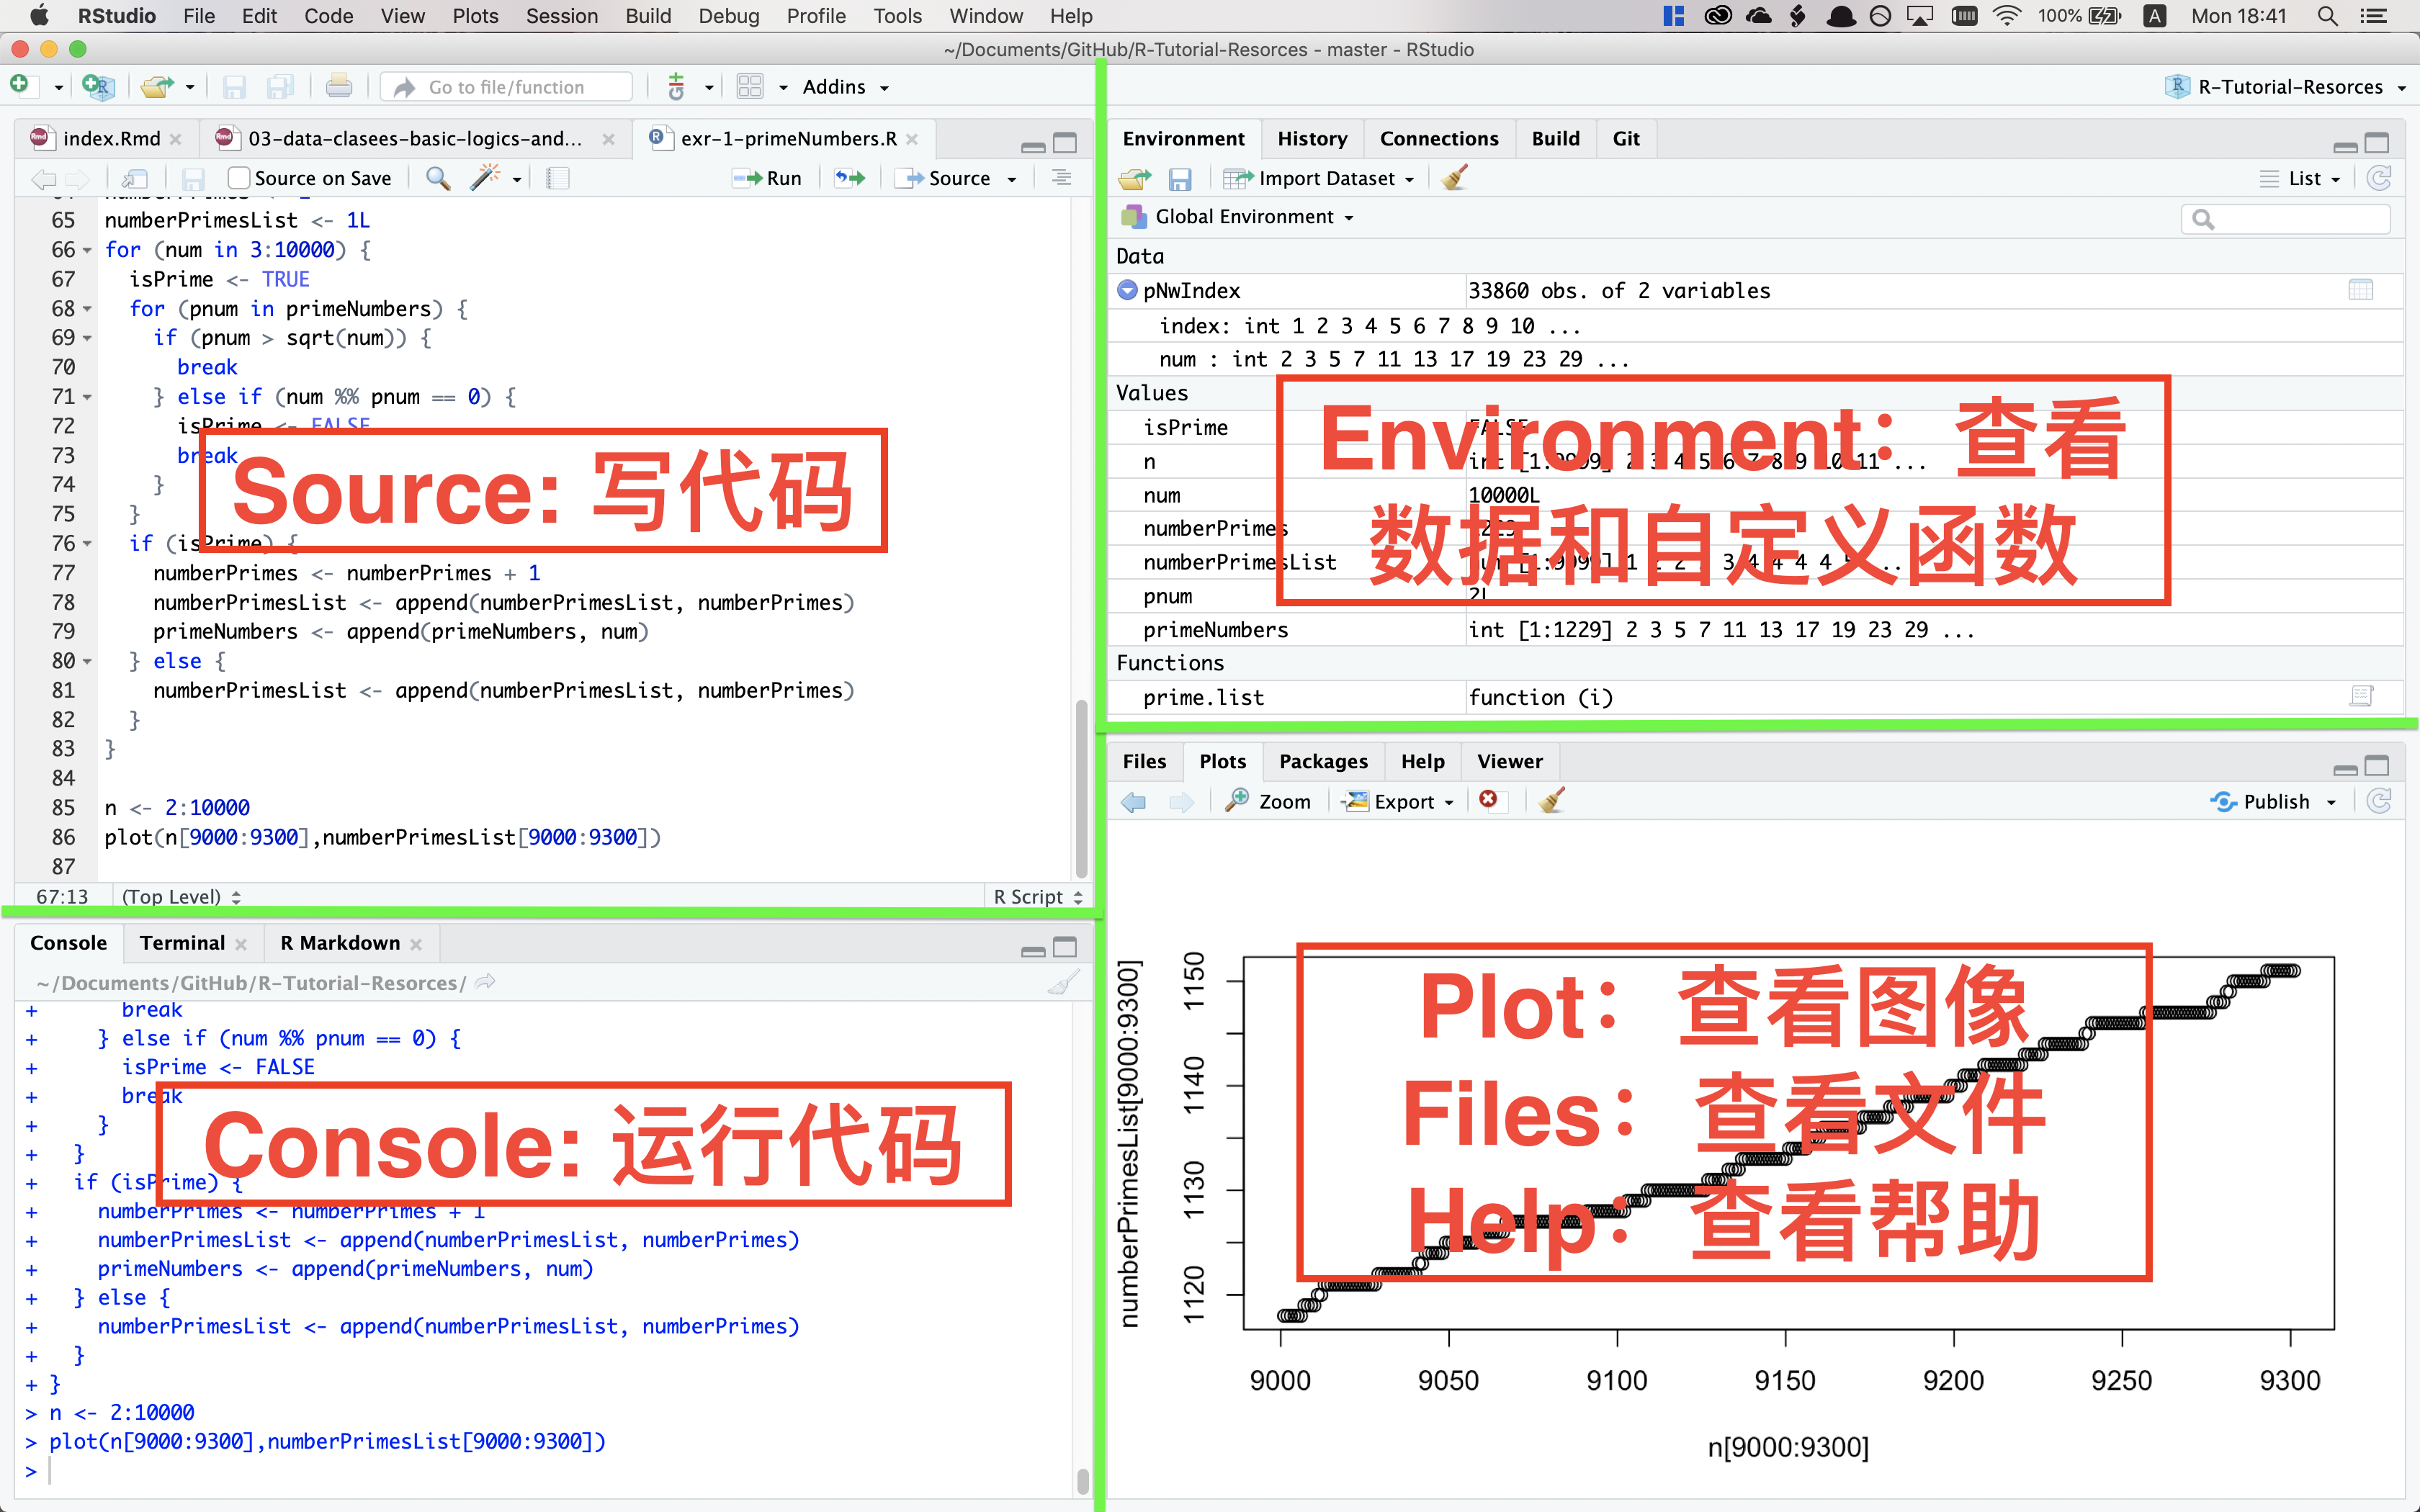
\includegraphics[width=46.67in]{img/01-interface}

\hypertarget{console}{%
\subsection{左下角:Console(控制台)}\label{console}}

Console是执行代码的地方。试试在里面输入\texttt{1\ +\ 1}并按回车以执行。

\hypertarget{source}{%
\subsection{左上角:Source(源)}\label{source}}

Source是写代码的地方。请看第\ref{manage}节。

这个位置也是用来查看文件和数据的地方。试试在console中执行\texttt{View(airquality)}或\texttt{library(help\ =\ "stats")}.

\hypertarget{environment}{%
\subsection{右上角:Environment(环境),}\label{environment}}

Environment 是一个列表,显示了所有当前工作环境中所有的变量(``values''和``data'')和自定义的函数(functions)。

History(历史)和 Connections(连接)不太常使用。

\hypertarget{plotshelpfilespackages}{%
\subsection{右下角:Plots(绘图),Help(帮助),Files(文件)和Packages(包)}\label{plotshelpfilespackages}}

Plots是预览图像的区域。试试在console中执行\texttt{hist(rnorm(10000))}.

Help是查看帮助文件的区域。试试在console中执行\texttt{?hist}或\texttt{?norm}.

Files是查看文件的区域,默认显示工作目录 (working directory)。

Packages是安装/查看/更新packages(包)的区域。详情请看第\ref{packages}章。

\section{基本操作}

\subsection{执行代码}

试着在console里输入\texttt{1\ +\ 1},并按回车以执行。你的console会显示:

\begin{verbatim}
> 1 + 1
[1] 2
\end{verbatim}

其中\texttt{2}是计算结果, \texttt{{[}1{]}}是索引,在第\ref{indexing}节有解释。\texttt{\textgreater{}\ 1\ +\ 1}是input,\texttt{{[}1{]}\ 2}是output.

还是用\texttt{1\ +\ 1}举例,在本书中,对于input和output的展示格式是这样的:

\begin{Shaded}
\begin{Highlighting}[]
\DecValTok{1}\OperatorTok{+}\DecValTok{1}
\end{Highlighting}
\end{Shaded}

\begin{verbatim}
## [1] 2
\end{verbatim}

注意input中的\texttt{\textgreater{}}被省略了,这意味着你可以直接把代码从本书复制到你的console并按回车执行(因为console本身自带了\texttt{\textgreater{}}),类似地,你从其他各种网站上找到的说明书,教程和论坛帖子中看到的R代码,大多数也都是这种形式呈现,便于复制粘贴。

再来一个例子,试着在console里输入(或者复制)以下代码并执行:

\begin{Shaded}
\begin{Highlighting}[]
\KeywordTok{attach}\NormalTok{(airquality)}
\end{Highlighting}
\end{Shaded}

\begin{verbatim}
## The following objects are masked from airquality (pos = 12):
## 
##     Day, Month, Ozone, Solar.R, Temp, Wind
\end{verbatim}

\begin{Shaded}
\begin{Highlighting}[]
\KeywordTok{plot}\NormalTok{(Wind, Ozone, }\DataTypeTok{main =} \StringTok{"Ozone and Wind in New York City"}\NormalTok{, }\DataTypeTok{pch =} \DecValTok{20}\NormalTok{)}
\NormalTok{model <-}\StringTok{ }\KeywordTok{lm}\NormalTok{(Ozone }\OperatorTok{~}\StringTok{ }\NormalTok{Wind, airquality)}
\KeywordTok{abline}\NormalTok{(model, }\DataTypeTok{lwd =} \DecValTok{2}\NormalTok{)}
\end{Highlighting}
\end{Shaded}

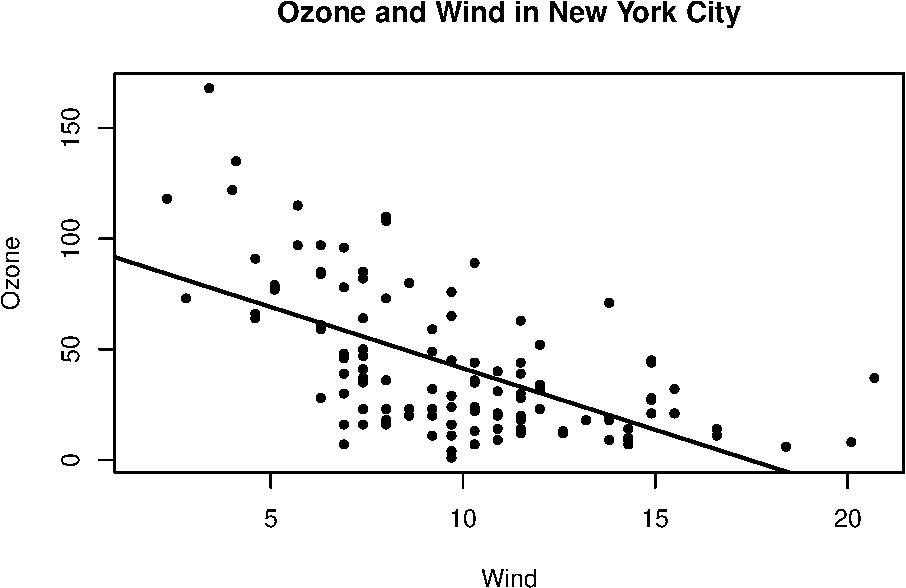
\includegraphics{R与tidyverse——数据分析入门_files/figure-latex/unnamed-chunk-4-1.pdf}

可以看到,在plots区,生成了一副漂亮的图。(先别在意每行代码具体的作用,在之后的章节我会一一讲述)

这时,把RStudio关掉,再重新启动,你会发现你的图没了。因此我们需要记录和管理代码。

\hypertarget{manage}{%
\subsection{记录和管理代码}\label{manage}}

初学者经常会在console里写代码,或者从别处复制代码,并执行。这对于一次性的计算(比如写统计学作业时用R来算线性回归的参数)很方便,但是如果你想保存你的工作,你需要把它们记录在R script文件里。如果你的工作比较复杂,比如有一个excel表格作为数据源,然后在R中用不同的方法分析,导出图表,这时候你会希望这些文件都集中在一起。你可以使用R Project来管理它们。

\hypertarget{r-project}{%
\subsubsection{创建R Project}\label{r-project}}

\begin{enumerate}
\def\labelenumi{\arabic{enumi}.}
\tightlist
\item
  左上角File \textgreater{} New Project
\item
  点选New Directory \textgreater{} New Project
\item
  输入名称和目录并Create Project
\end{enumerate}

\hypertarget{r-project}{%
\subsubsection{使用R Project}\label{r-project}}

在创建R project的文件夹中打开\texttt{.Rproj}文件。或者,RStudio启动的时候默认会使用上一次所使用的R project.

随后,你在RStudio中做的所有工作都会被保存到\texttt{.Rproj}所在的这个文件夹(正规的说法是``工作目录'' (working directory))。比如,在console中执行:

\begin{Shaded}
\begin{Highlighting}[]
\KeywordTok{pdf}\NormalTok{(}\StringTok{"normalDistrubution.pdf"}\NormalTok{)}
\KeywordTok{curve}\NormalTok{(}\KeywordTok{dnorm}\NormalTok{(x),}\OperatorTok{-}\DecValTok{5}\NormalTok{,}\DecValTok{5}\NormalTok{)}
\KeywordTok{dev.off}\NormalTok{()}
\end{Highlighting}
\end{Shaded}

一个正态分布的图像便以pdf格式保存在了工作目录。你可以在系统的文件管理器中,或是在RStudio右下角File面板中找到。

\hypertarget{r-script}{%
\subsection{写/保存/运行R script}\label{r-script}}

在console中运行代码,代码得不到保存。代码需保存在R script文件(后缀为\texttt{.R})里。

\texttt{Ctrl}+\texttt{Shift}+\texttt{N}(Mac是\texttt{command}+\texttt{shift}+\texttt{N})以创建新R script.

然后就可以写R script. 合理使用换行可以使你的代码更易读。\texttt{\#}是注释符号。每行第一个\texttt{\#}以及之后的内容不会被执行。之前的例子,可以写成这样:

\begin{Shaded}
\begin{Highlighting}[]
\CommentTok{# 读取数据}
\KeywordTok{attach}\NormalTok{(airquality)}

\CommentTok{# 绘图}
\KeywordTok{plot}\NormalTok{(Wind, Ozone, }\CommentTok{# x轴和y轴}
     \DataTypeTok{main =} \StringTok{"Ozone and Wind in New York City"}\NormalTok{, }\CommentTok{# 标题}
     \DataTypeTok{pch =} \DecValTok{20}\NormalTok{) }\CommentTok{# 使用实心圆点}
\NormalTok{model <-}\StringTok{ }\KeywordTok{lm}\NormalTok{(Ozone }\OperatorTok{~}\StringTok{ }\NormalTok{Wind, airquality) }\CommentTok{# 线性回归模型}
\KeywordTok{abline}\NormalTok{(model, }\DataTypeTok{lwd =} \DecValTok{2}\NormalTok{) }\CommentTok{# 回归线}
\end{Highlighting}
\end{Shaded}

\texttt{Ctrl}+\texttt{Enter} (\texttt{command}+\texttt{return})以执行一``句''代码(比如上面的例子中,从\texttt{plot(Wind...}到\texttt{pch\ =\ 20)}有三行,但是它是一``句'')。

\texttt{Ctrl}+\texttt{Shift}+\texttt{Enter} (\texttt{command}+\texttt{shift}+\texttt{return})以从头到尾执行所有代码。

试试复制并执行以上代码吧。

\texttt{Ctrl}+\texttt{S} (\texttt{command}+\texttt{S})以保存R script. 保存后会在工作目录找到你新保存的\texttt{.R}文件。重新启动RStudio的时候,便可以打开对应的R script文件以重复/继续之前的工作。

\subsection{关于换行}

Console 中每个命令开头的\texttt{\textgreater{}}叫做prompt(命令提示符),当它出现在你所编辑的那一行的开头时,按下回车的时候那行的命令才会被执行。有时候它会消失,这时候按\texttt{esc}可以将其恢复。

prompt消失的主要原因是你的代码没有写完,比如括号不完整:

\begin{verbatim}
> 2+(3+4
\end{verbatim}

这时你按回车,它会显示:

\begin{verbatim}
> 2+(3+4
+
\end{verbatim}

\texttt{+}号是在提示代码没写完整。这时你把括号补上再按回车:

\begin{verbatim}
> 2+(3+4
+ )
\end{verbatim}

\begin{verbatim}
[1] 9
\end{verbatim}

便可以完成计算。

这意味着我们可以把一条很长的命令分成很多行。比如我们可以写这样的代码(在R script编辑器中!)

\begin{Shaded}
\begin{Highlighting}[]
\ControlFlowTok{if}\NormalTok{(}\OtherTok{TRUE}\NormalTok{)\{}
  \KeywordTok{print}\NormalTok{(}\DecValTok{2}\NormalTok{)}
\NormalTok{\} }\ControlFlowTok{else}\NormalTok{\{}
  \KeywordTok{print}\NormalTok{(}\DecValTok{3}\NormalTok{)}
\NormalTok{\}}
\end{Highlighting}
\end{Shaded}

然后\texttt{Ctrl}+\texttt{Enter}执行。你会发现在console中,从第二行开始每行开头都有一个\texttt{+}号。

\hypertarget{packages}{%
\chapter{安装和使用packages (包)}\label{packages}}

\hypertarget{package}{%
\section{Package是什么,为什么使用它们?}\label{package}}

Package是别人写好的在R中运行的程序(以及附带的数据和文档),你可以免费安装和使用它们。

Packages可以增加在基础R语言中没有的功能,可以精简你代码的语句,或是提升使用体验。比如有个叫做\texttt{tikzDevice}的package可以将R中的图表导出成tikz语法的矢量图,方便在LaTeX中使用。本书的编写和排版也是使用R中的一个叫做\texttt{bookdown}的package完成的(真的超棒).

这个课程主要是学习\texttt{tidyverse}这个package,

\hypertarget{packages}{%
\section{如何安装packages}\label{packages}}

首先我们安装tidyverse(\textbf{很重要,本书接下来的部分都要使用这个package}):

\begin{Shaded}
\begin{Highlighting}[]
\KeywordTok{install.packages}\NormalTok{(}\StringTok{"tidyverse"}\NormalTok{)}
\end{Highlighting}
\end{Shaded}

在console中运行以上代码,R就会从\href{https://cran.r-project.org}{CRAN}中下载tidyverse并安装到你电脑上的默认位置。因此安装packages需要网络连接。

如果想安装多个packages,你可以一行一行地安装,或是把多个packages的名字合成一列,同时安装,比如:

\begin{Shaded}
\begin{Highlighting}[]
\KeywordTok{install.packages}\NormalTok{(}\KeywordTok{c}\NormalTok{(}\StringTok{"nycflights13"}\NormalTok{, }\StringTok{"gapminder"}\NormalTok{, }\StringTok{"Lahman"}\NormalTok{)}
\end{Highlighting}
\end{Shaded}

绝大多数的packages都能用这个方法安装,因为它们是被存储在CRAN上的。Bioconductor packages请看第\ref{Bioconductor}节。

\hypertarget{packages}{%
\section{如何使用packages}\label{packages}}

安装packages后,有两种方法使用它们。以\texttt{tidyverse}为例:

\begin{Shaded}
\begin{Highlighting}[]
\KeywordTok{library}\NormalTok{(}\StringTok{'tidyverse'}\NormalTok{)}
\end{Highlighting}
\end{Shaded}

或

\begin{Shaded}
\begin{Highlighting}[]
\KeywordTok{require}\NormalTok{(}\StringTok{'tidyverse'}\NormalTok{)}
\end{Highlighting}
\end{Shaded}

两者的效果很大程度上都是一样的,都可以用来读取\textbf{单个}package。它们的不同,以及如何通过一行指令读取多个packages,请参看第\ref{require-and-library}节。

每次重启R的时候,上一次使用的packages都会被清空,所以需要重新读取。因此我们要在R script里面记录此script需要使用的packages(这个特性可以帮助你养成好习惯:当你把你的代码分享给别人的时候,要保证在别人的电脑上也能正常运行,就必须要指明要使用哪些packages)

\section{其它}

这小节是一些不重要的内容,因此\textbf{可酌情跳到下一章(第\ref{vectors-logicals-and-functions}章。}

\hypertarget{require-and-library}{%
\subsection{\texorpdfstring{\texttt{library()}和\texttt{require}的区别;如何使用一行指令读取多个packages}{library()和require的区别;如何使用一行指令读取多个packages}}\label{require-and-library}}

\begin{enumerate}
\def\labelenumi{\arabic{enumi}.}
\tightlist
\item
  \texttt{require()}会返回一个逻辑值。如果package读取成功,会返回\texttt{TRUE},反之则返回\texttt{FALSE}.
\item
  \texttt{library()}如果读取试图读取不存在的package,会直接造成错误(error),而\texttt{require()}不会造成错误,只会产生一个警告(warning).
\end{enumerate}

这意味着\texttt{require()}可以用来同时读取多个packages:

\begin{Shaded}
\begin{Highlighting}[]
\KeywordTok{lapply}\NormalTok{(}\KeywordTok{c}\NormalTok{(}\StringTok{"dplyr"}\NormalTok{,}\StringTok{"ggplot2"}\NormalTok{), require, }\DataTypeTok{character.only =} \OtherTok{TRUE}\NormalTok{)}
\end{Highlighting}
\end{Shaded}

\begin{verbatim}
## [[1]]
## [1] TRUE
## 
## [[2]]
## [1] TRUE
\end{verbatim}

或者更精简一点,

\begin{Shaded}
\begin{Highlighting}[]
\KeywordTok{lapply}\NormalTok{(}\KeywordTok{c}\NormalTok{(}\StringTok{"dplyr"}\NormalTok{,}\StringTok{"ggplot2"}\NormalTok{), require, }\DataTypeTok{c =}\NormalTok{ T)}
\end{Highlighting}
\end{Shaded}

\begin{verbatim}
## [[1]]
## [1] TRUE
## 
## [[2]]
## [1] TRUE
\end{verbatim}

\hypertarget{Bioconductor}{%
\subsection{安装Bioconductor packages}\label{Bioconductor}}

\href{https://bioconductor.org}{Bioconductor}是一系列用于生物信息学的R packages. 截止2019年7月2日,共有1741个可用的bioconductor packages. 它们没有被存储在CRAN上,因此需要用特殊的方法安装。首先,安装一系列Bioconductor的核心packages(可能需要几分钟):

\begin{Shaded}
\begin{Highlighting}[]
\KeywordTok{source}\NormalTok{(}\StringTok{"http://bioconductor.org/biocLite.R"}\NormalTok{)}
\KeywordTok{biocLite}\NormalTok{()}
\end{Highlighting}
\end{Shaded}

然后,通过\texttt{biocLite()}函数安装其它packages,比如:

\begin{Shaded}
\begin{Highlighting}[]
\KeywordTok{biocLite}\NormalTok{(}\StringTok{"RforProteomics"}\NormalTok{)}
\end{Highlighting}
\end{Shaded}

\hypertarget{vectors-logicals-and-functions}{%
\chapter{向量,逻辑,循环和函数}\label{vectors-logicals-and-functions}}

\emph{注意,R中的变量名/自定义函数名不能以数字和特殊符号开头,中间只能使用"\_``和''."作为特殊符号}\footnote{如果非要违反规则,可以使用转义符号\texttt{\textbackslash{}\textasciigrave{}\textasciigrave{},比如可以\textasciigrave{}\textasciigrave{}}4foo\%b=a+r` \textless{}- 50 ``}

\section{向量的概念,操作和优越性}

R没有标量,它通过各种类型的向量 (vector)来存储数据。

\hypertarget{create-vector}{%
\subsection{创建向量(赋值)}\label{create-vector}}

与很多其他的计算机语言不同,在R中,\texttt{\textless{}-}(像一个小箭头)用于给\textbf{向量,数据框和函数}赋值(即在每行的开头)。在RStudio中,可以用\texttt{Alt}+\texttt{-} (Mac是 \texttt{option}+\texttt{-}) 这个快捷键打出这个符号。

\begin{Shaded}
\begin{Highlighting}[]
\NormalTok{x <-}\StringTok{ }\DecValTok{2}
\NormalTok{x}
\end{Highlighting}
\end{Shaded}

\begin{verbatim}
## [1] 2
\end{verbatim}

虽然\texttt{=}也可以用,但是绝大多数R用户还是采用标准的\texttt{\textless{}-}符号,而\texttt{=}则用于给\textbf{函数的参数}赋值。

要创建一个多元素的向量,需要用到\texttt{c()} (concatenate)函数:

\begin{Shaded}
\begin{Highlighting}[]
\NormalTok{nums <-}\StringTok{ }\KeywordTok{c}\NormalTok{(}\DecValTok{1}\NormalTok{,}\DecValTok{45}\NormalTok{,}\DecValTok{78}\NormalTok{)}
\NormalTok{cities <-}\StringTok{ }\KeywordTok{c}\NormalTok{(}\StringTok{"Zürich", "}\NormalTok{上海}\StringTok{", "}\NormalTok{Tehrān}\StringTok{")}
\StringTok{nums}
\end{Highlighting}
\end{Shaded}

\begin{verbatim}
## [1]  1 45 78
\end{verbatim}

\begin{Shaded}
\begin{Highlighting}[]
\NormalTok{cities}
\end{Highlighting}
\end{Shaded}

\begin{verbatim}
## [1] "Zürich" "上海"   "Tehrān"
\end{verbatim}

通过\texttt{length()}函数,可以查看向量的长度。

\begin{Shaded}
\begin{Highlighting}[]
\KeywordTok{length}\NormalTok{(nums)}
\end{Highlighting}
\end{Shaded}

\begin{verbatim}
## [1] 3
\end{verbatim}

\begin{Shaded}
\begin{Highlighting}[]
\CommentTok{#如果无后续使用,没必要赋值一个变量;c(...)的计算结果就是一个向量,并直接传给`length()`函数}
\KeywordTok{length}\NormalTok{(}\KeywordTok{c}\NormalTok{(}\StringTok{"Guten Morgen"}\NormalTok{)) }
\end{Highlighting}
\end{Shaded}

\begin{verbatim}
## [1] 1
\end{verbatim}

(每个被引号包围的一串字符,都只算做一个元素,因此长度为1;多元素的向量请看第\ref{create-vector}节)

还是通过\texttt{c()}函数,可以把多个向量拼接起来:

\begin{Shaded}
\begin{Highlighting}[]
\NormalTok{cities_}\DecValTok{1}\NormalTok{ <-}\StringTok{ }\KeywordTok{c}\NormalTok{(}\StringTok{"Zürich", "}\NormalTok{上海}\StringTok{", "}\NormalTok{Tehrān}\StringTok{")}
\StringTok{cities_2 <- c("}\NormalTok{大阪}\StringTok{", "}\NormalTok{Poznań}\StringTok{", "}\NormalTok{Екатеринбу́рг}\StringTok{")}

\StringTok{cities <- c(cities_1, cities_2, c("}\NormalTok{Jyväskylä}\StringTok{", "}\NormalTok{부산}\StringTok{", "}\NormalTok{เชียงใหม่}\StringTok{"))}

\StringTok{cities}
\end{Highlighting}
\end{Shaded}

\begin{verbatim}
## [1] "Zürich"       "上海"         "Tehrān"       "大阪"        
## [5] "Poznań"       "Екатеринбу́рг" "Jyväskylä"    "부산"        
## [9] "เชียงใหม่"
\end{verbatim}

\hypertarget{indexing}{%
\subsection{索引/取子集 (indexing/subsetting)}\label{indexing}}

索引 (index)就是一个元素在向量中的位置。R是从1开始索引的,即索引为1的元素是第一个元素(因此用熟了Python和C可能会有些不适应)。在向量后方使用方括号进行取子集运算(即抓取索引为对应数字的元素;虽然subsetting翻译成``取子集''有点怪,但是没毛病;不知大家有没有更好的翻译方法,或是不翻译更好)。

\begin{Shaded}
\begin{Highlighting}[]
\NormalTok{x <-}\StringTok{ }\KeywordTok{c}\NormalTok{(}\StringTok{"one"}\NormalTok{, }\StringTok{"two"}\NormalTok{, }\StringTok{"three"}\NormalTok{, }\StringTok{"four"}\NormalTok{, }\StringTok{"five"}\NormalTok{, }\StringTok{"six"}\NormalTok{, }\StringTok{"seven"}\NormalTok{, }\StringTok{"eight"}\NormalTok{, }\StringTok{"nine"}\NormalTok{)}
\NormalTok{x[}\DecValTok{3}\NormalTok{]}
\end{Highlighting}
\end{Shaded}

\begin{verbatim}
## [1] "three"
\end{verbatim}

可以在方括号中使用另一个向量抓取多个元素:

\begin{Shaded}
\begin{Highlighting}[]
\NormalTok{x[}\KeywordTok{c}\NormalTok{(}\DecValTok{2}\NormalTok{,}\DecValTok{5}\NormalTok{,}\DecValTok{9}\NormalTok{)] }\CommentTok{# 第2个,第5个,第9个元素}
\end{Highlighting}
\end{Shaded}

\begin{verbatim}
## [1] "two"  "five" "nine"
\end{verbatim}

经常,我们会抓取几个连续的元素。如果想知道方法,请继续往下看。

\subsection{生成器}

有时候我们需要其元素按一定规律排列的向量,这时,相对于一个个手动输入,有更方便的方法:

\subsubsection{连续整数}

\begin{Shaded}
\begin{Highlighting}[]
\DecValTok{1}\OperatorTok{:}\DecValTok{10} \CommentTok{#从左边的数(包含)到右边的数(包含),即1:10}
\end{Highlighting}
\end{Shaded}

\begin{verbatim}
##  [1]  1  2  3  4  5  6  7  8  9 10
\end{verbatim}

这时,你应该会有个大胆的想法:

\begin{Shaded}
\begin{Highlighting}[]
\NormalTok{x[}\DecValTok{3}\OperatorTok{:}\DecValTok{6}\NormalTok{]}
\end{Highlighting}
\end{Shaded}

\begin{verbatim}
## [1] "three" "four"  "five"  "six"
\end{verbatim}

没错就是这么用的,而且极为常用。

当元素比较多的时候:

\begin{Shaded}
\begin{Highlighting}[]
\NormalTok{y <-}\StringTok{ }\DecValTok{7}\OperatorTok{:}\DecValTok{103} \CommentTok{#复习一下赋值}
\NormalTok{y}
\end{Highlighting}
\end{Shaded}

\begin{verbatim}
##  [1]   7   8   9  10  11  12  13  14  15  16  17  18  19  20  21  22  23
## [18]  24  25  26  27  28  29  30  31  32  33  34  35  36  37  38  39  40
## [35]  41  42  43  44  45  46  47  48  49  50  51  52  53  54  55  56  57
## [52]  58  59  60  61  62  63  64  65  66  67  68  69  70  71  72  73  74
## [69]  75  76  77  78  79  80  81  82  83  84  85  86  87  88  89  90  91
## [86]  92  93  94  95  96  97  98  99 100 101 102 103
\end{verbatim}

注意到了左边方括号中的数字了吗?它们正是所对应的那一行第一个元素的索引。

下面的内容可能有点偏,\textbf{可以酌情从这里跳到第\ref{youyuexing}节。}

\hypertarget{rep}{%
\subsubsection{\texorpdfstring{复读机\texttt{rep()}}{复读机rep()}}\label{rep}}

\begin{Shaded}
\begin{Highlighting}[]
\KeywordTok{rep}\NormalTok{(}\KeywordTok{c}\NormalTok{(}\DecValTok{0}\NormalTok{, }\DecValTok{7}\NormalTok{, }\DecValTok{6}\NormalTok{, }\DecValTok{0}\NormalTok{), }\DecValTok{4}\NormalTok{) }\CommentTok{# 把[0, 7, 6, 0]重复4遍}
\end{Highlighting}
\end{Shaded}

\begin{verbatim}
##  [1] 0 7 6 0 0 7 6 0 0 7 6 0 0 7 6 0
\end{verbatim}

\hypertarget{-seq}{%
\subsubsection{\texorpdfstring{等差数列: \texttt{seq()}}{等差数列: seq()}}\label{-seq}}

公差确定时:

\begin{Shaded}
\begin{Highlighting}[]
\KeywordTok{seq}\NormalTok{(}\DecValTok{0}\NormalTok{, }\DecValTok{15}\NormalTok{, }\FloatTok{2.5}\NormalTok{) }\CommentTok{# 其实是`seq(from = 0, to = 50, by = 5)`的简写}
\end{Highlighting}
\end{Shaded}

\begin{verbatim}
## [1]  0.0  2.5  5.0  7.5 10.0 12.5 15.0
\end{verbatim}

长度确定时:

\begin{Shaded}
\begin{Highlighting}[]
 \KeywordTok{seq}\NormalTok{(}\DecValTok{0}\NormalTok{, }\DecValTok{50}\NormalTok{, }\DataTypeTok{length.out =} \DecValTok{11}\NormalTok{) }\CommentTok{# 其实是`seq(from = 0, to = 50, length.out = 11)`的简写}
\end{Highlighting}
\end{Shaded}

\begin{verbatim}
##  [1]  0  5 10 15 20 25 30 35 40 45 50
\end{verbatim}

\subsubsection{随机数:}

连续型均匀分布随机数用\texttt{runif(n,\ min,\ max)},n是数量,min是最小值,max是最大值。默认min为0,max为1。

\begin{Shaded}
\begin{Highlighting}[]
\NormalTok{x_unif <-}\StringTok{ }\KeywordTok{runif}\NormalTok{(}\DecValTok{100000}\NormalTok{, }\DecValTok{40}\NormalTok{, }\DecValTok{60}\NormalTok{) }\CommentTok{# 生成100000个40到60之间,连续均匀分布的的随机数}
\KeywordTok{hist}\NormalTok{(x_unif) }\CommentTok{# 画直方图}
\end{Highlighting}
\end{Shaded}

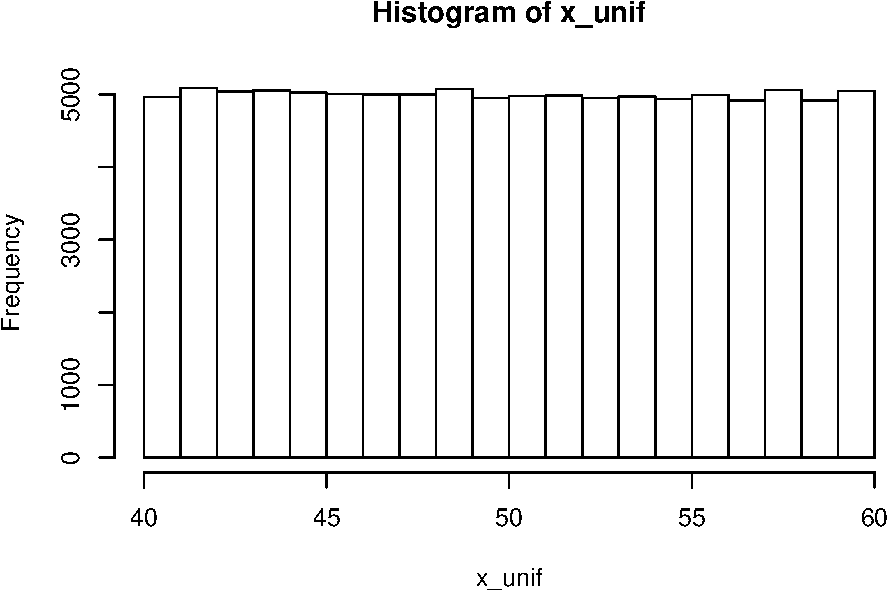
\includegraphics{R与tidyverse——数据分析入门_files/figure-latex/unnamed-chunk-28-1.pdf}

正态分布随机数用\texttt{rnorm(n,\ mean,\ sd)}, 三个参数分别为数量,平均值,标准差。默认mean为0,sd为1。

\begin{Shaded}
\begin{Highlighting}[]
\NormalTok{x_norm <-}\StringTok{ }\KeywordTok{rnorm}\NormalTok{(}\DecValTok{100000}\NormalTok{, }\DecValTok{250}\NormalTok{, }\DecValTok{20}\NormalTok{) }\CommentTok{# 按照平均值为250,标准差为20的正态分布的概率密度函数生成100000个随机数}
\KeywordTok{hist}\NormalTok{(x_norm) }\CommentTok{# 画直方图}
\end{Highlighting}
\end{Shaded}

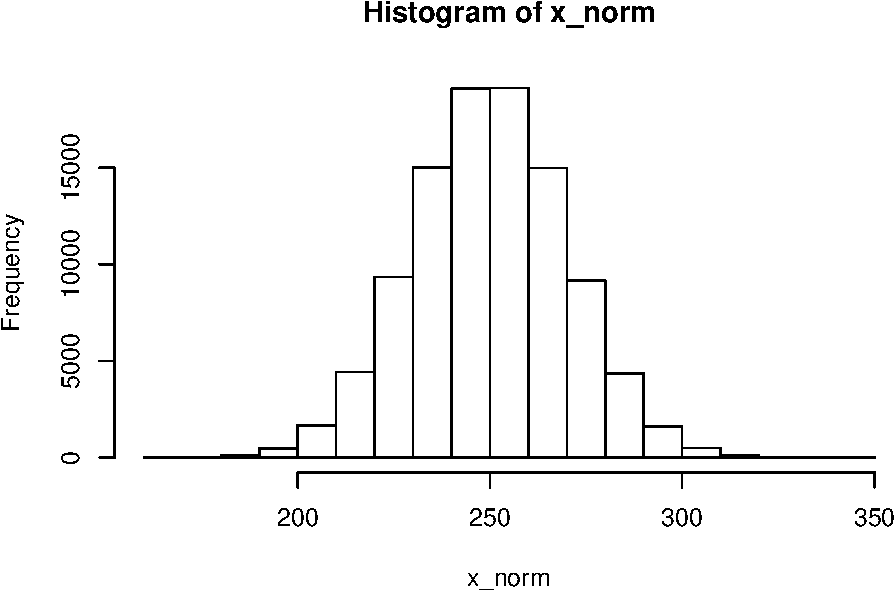
\includegraphics{R与tidyverse——数据分析入门_files/figure-latex/unnamed-chunk-29-1.pdf}

\subsection{向量的其它操作}

\hypertarget{sort-rankorder}{%
\subsubsection{\texorpdfstring{\texttt{sort()}, \texttt{rank()}和\texttt{order()}}{sort(), rank()和order()}}\label{sort-rankorder}}

\hypertarget{youyuexing}{%
\subsection{R向量的优越性}\label{youyuexing}}

R中的向量(矩阵和数列也是)的各种计算默认都是逐元素 (elementwise)的。比如:

\begin{Shaded}
\begin{Highlighting}[]
\NormalTok{x <-}\StringTok{ }\KeywordTok{c}\NormalTok{(}\DecValTok{4}\NormalTok{, }\DecValTok{9}\NormalTok{, }\DecValTok{25}\NormalTok{)}
\NormalTok{y <-}\StringTok{ }\KeywordTok{c}\NormalTok{(}\DecValTok{8}\NormalTok{, }\DecValTok{6}\NormalTok{, }\DecValTok{3}\NormalTok{)}
\NormalTok{x }\OperatorTok{+}\StringTok{ }\NormalTok{y}
\end{Highlighting}
\end{Shaded}

\begin{verbatim}
## [1] 12 15 28
\end{verbatim}

\begin{Shaded}
\begin{Highlighting}[]
\NormalTok{x }\OperatorTok{*}\StringTok{ }\NormalTok{y }\CommentTok{# 在matlab中这样乘是不行的,要用`.*`,除法也是}
\end{Highlighting}
\end{Shaded}

\begin{verbatim}
## [1] 32 54 75
\end{verbatim}

\begin{Shaded}
\begin{Highlighting}[]
\KeywordTok{sqrt}\NormalTok{(x)}
\end{Highlighting}
\end{Shaded}

\begin{verbatim}
## [1] 2 3 5
\end{verbatim}

相比于常用的编程语言,省去了for循环;相比于matlab的默认矩阵乘法,逐元素乘法在数据处理中更有用。

\hypertarget{-data-types}{%
\section{数据类型 (Data Types)}\label{-data-types}}

向量所存储的的数据类型有:

\begin{longtable}[]{@{}lll@{}}
\toprule
类型 & 含义与说明 & 例子\tabularnewline
\midrule
\endhead
numeric & 浮点数向量 & \texttt{3}, \texttt{0.5}, \texttt{sqrt(2)}, \texttt{NaN}, \texttt{Inf}\tabularnewline
integer & 整数向量 & \texttt{3L}, \texttt{100L}\tabularnewline
character & 字符向量;需被引号包围 & \texttt{"1"}, \texttt{"\$"}, \texttt{"你好"}\tabularnewline
logical & 逻辑向量 & \texttt{TRUE}, \texttt{FALSE}, \texttt{NA}\tabularnewline
complex & 复数向量 & \texttt{3+5i}, \texttt{1i}, \texttt{1+0i}\tabularnewline
\bottomrule
\end{longtable}

通过\texttt{class()}函数,可以查看向量的类型。

\begin{Shaded}
\begin{Highlighting}[]
\KeywordTok{class}\NormalTok{(}\StringTok{"早上好"}\NormalTok{)}
\end{Highlighting}
\end{Shaded}

\begin{verbatim}
## [1] "character"
\end{verbatim}

(除此之外,\texttt{typeof()}, \texttt{mode()}, \texttt{storage.mode()}这三个函数的功能与\texttt{class()}类似,但有重要的区别;为避免造成困惑,此处不展开讨论)。

\section{数学表达和运算}

\subsection{数的表达}

\subsubsection{浮点数}

除非指定作为整数(见下),在R中所有的数都被存储为双精度浮点数的格式 (double-precision floating-point format),其\texttt{class}为\texttt{numeric}。

\begin{Shaded}
\begin{Highlighting}[]
\KeywordTok{class}\NormalTok{(}\DecValTok{3}\NormalTok{)}
\end{Highlighting}
\end{Shaded}

\begin{verbatim}
## [1] "numeric"
\end{verbatim}

这会导致一些有趣的现象,比如\((\sqrt{3})^2 \neq 3\):\sout{(强迫症患者浑身难受)}

\begin{Shaded}
\begin{Highlighting}[]
\KeywordTok{sqrt}\NormalTok{(}\DecValTok{3}\NormalTok{)}\OperatorTok{^}\DecValTok{2-3}
\end{Highlighting}
\end{Shaded}

\begin{verbatim}
## [1] -4.440892e-16
\end{verbatim}

浮点数的计算比精确数的计算快很多。如果你是第一次接触浮点数,可能会觉得它不可靠,其实不然。在绝大多数情况下,牺牲的这一点点精度并不会影响计算结果(我们的结果所需要的有效数字一般不会超过10位;只有当两个非常,非常大且数值相近对数字相减才会出现较大的误差)。

\texttt{NaN}(非数)和\texttt{Inf}(无限大)也是浮点数!

\begin{Shaded}
\begin{Highlighting}[]
\KeywordTok{class}\NormalTok{(}\OtherTok{NaN}\NormalTok{)}
\end{Highlighting}
\end{Shaded}

\begin{verbatim}
## [1] "numeric"
\end{verbatim}

\begin{Shaded}
\begin{Highlighting}[]
\KeywordTok{class}\NormalTok{(}\OtherTok{Inf}\NormalTok{)}
\end{Highlighting}
\end{Shaded}

\begin{verbatim}
## [1] "numeric"
\end{verbatim}

\subsubsection{科学计数法}

在R中可以使用科学计数法(\texttt{AeB}\(= A \times 10^B\)),比如:

\begin{Shaded}
\begin{Highlighting}[]
\FloatTok{3.1e5}
\end{Highlighting}
\end{Shaded}

\begin{verbatim}
## [1] 310000
\end{verbatim}

\begin{Shaded}
\begin{Highlighting}[]
\FloatTok{-1.2e-4+1.1e-5}
\end{Highlighting}
\end{Shaded}

\begin{verbatim}
## [1] -0.000109
\end{verbatim}

\subsubsection{整数}

整数的class为\texttt{integer}。有两种常见的方法创建整数:
1)在数后面加上\texttt{L};

\begin{Shaded}
\begin{Highlighting}[]
\KeywordTok{class}\NormalTok{(}\DecValTok{2}\NormalTok{)}
\end{Highlighting}
\end{Shaded}

\begin{verbatim}
## [1] "numeric"
\end{verbatim}

\begin{Shaded}
\begin{Highlighting}[]
\KeywordTok{class}\NormalTok{(2L)}
\end{Highlighting}
\end{Shaded}

\begin{verbatim}
## [1] "integer"
\end{verbatim}

2)创建数列

\begin{Shaded}
\begin{Highlighting}[]
\DecValTok{1}\OperatorTok{:}\DecValTok{10} \CommentTok{#公差为1的整数向量生成器,包含最小值和最大值}
\end{Highlighting}
\end{Shaded}

\begin{verbatim}
##  [1]  1  2  3  4  5  6  7  8  9 10
\end{verbatim}

\begin{Shaded}
\begin{Highlighting}[]
\KeywordTok{class}\NormalTok{(}\DecValTok{1}\OperatorTok{:}\DecValTok{10}\NormalTok{)}
\end{Highlighting}
\end{Shaded}

\begin{verbatim}
## [1] "integer"
\end{verbatim}

\begin{Shaded}
\begin{Highlighting}[]
\KeywordTok{seq}\NormalTok{(}\DecValTok{5}\NormalTok{,}\DecValTok{50}\NormalTok{,}\DecValTok{5}\NormalTok{) }\CommentTok{#自定义公差,首项,末项和公差可以不为整数}
\end{Highlighting}
\end{Shaded}

\begin{verbatim}
##  [1]  5 10 15 20 25 30 35 40 45 50
\end{verbatim}

\begin{Shaded}
\begin{Highlighting}[]
\KeywordTok{class}\NormalTok{(}\KeywordTok{seq}\NormalTok{(}\DecValTok{5}\NormalTok{,}\DecValTok{50}\NormalTok{,}\DecValTok{5}\NormalTok{)) }\CommentTok{#因此产生的是一个浮点数向量}
\end{Highlighting}
\end{Shaded}

\begin{verbatim}
## [1] "numeric"
\end{verbatim}

\begin{Shaded}
\begin{Highlighting}[]
\KeywordTok{seq}\NormalTok{(5L,50L,5L) }\CommentTok{#可以强制生成整数}
\end{Highlighting}
\end{Shaded}

\begin{verbatim}
##  [1]  5 10 15 20 25 30 35 40 45 50
\end{verbatim}

\begin{Shaded}
\begin{Highlighting}[]
\KeywordTok{class}\NormalTok{(}\KeywordTok{seq}\NormalTok{(5L,50L,5L)) }\CommentTok{#是�整数没错}
\end{Highlighting}
\end{Shaded}

\begin{verbatim}
## [1] "integer"
\end{verbatim}

整数最常见的用处是indexing(索引)。

\paragraph{整数变成浮点数的情况}

这一小段讲的比较细,\textbf{请酌情直接跳到下一节(\ref{arithmetic})。}

整数与整数之前的加,减,乘,求整数商,和求余数计算会得到整数,其他的运算都会得到浮点数,(阶乘(\texttt{factorial})也是,即便现实中不管怎么阶乘都不可能得到非整数):

\begin{Shaded}
\begin{Highlighting}[]
\KeywordTok{class}\NormalTok{(2L}\OperatorTok{+}\NormalTok{1L)}
\end{Highlighting}
\end{Shaded}

\begin{verbatim}
## [1] "integer"
\end{verbatim}

\begin{Shaded}
\begin{Highlighting}[]
\KeywordTok{class}\NormalTok{(2L}\OperatorTok{-}\NormalTok{1L)}
\end{Highlighting}
\end{Shaded}

\begin{verbatim}
## [1] "integer"
\end{verbatim}

\begin{Shaded}
\begin{Highlighting}[]
\KeywordTok{class}\NormalTok{(2L}\OperatorTok{*}\NormalTok{3L)}
\end{Highlighting}
\end{Shaded}

\begin{verbatim}
## [1] "integer"
\end{verbatim}

\begin{Shaded}
\begin{Highlighting}[]
\KeywordTok{class}\NormalTok{(17L}\OperatorTok\NormalTok{3L)}
\end{Highlighting}
\end{Shaded}

\begin{verbatim}
## [1] "integer"
\end{verbatim}

\begin{Shaded}
\begin{Highlighting}[]
\KeywordTok{class}\NormalTok{(17L}\OperatorTok\NormalTok{3L)}
\end{Highlighting}
\end{Shaded}

\begin{verbatim}
## [1] "integer"
\end{verbatim}

\begin{Shaded}
\begin{Highlighting}[]
\KeywordTok{class}\NormalTok{(1000L}\OperatorTok{/}\NormalTok{1L)}
\end{Highlighting}
\end{Shaded}

\begin{verbatim}
## [1] "numeric"
\end{verbatim}

\begin{Shaded}
\begin{Highlighting}[]
\KeywordTok{class}\NormalTok{(3L}\OperatorTok{^}\NormalTok{4L)}
\end{Highlighting}
\end{Shaded}

\begin{verbatim}
## [1] "numeric"
\end{verbatim}

\begin{Shaded}
\begin{Highlighting}[]
\KeywordTok{class}\NormalTok{(}\KeywordTok{sqrt}\NormalTok{(4L))}
\end{Highlighting}
\end{Shaded}

\begin{verbatim}
## [1] "numeric"
\end{verbatim}

\begin{Shaded}
\begin{Highlighting}[]
\KeywordTok{class}\NormalTok{(}\KeywordTok{log}\NormalTok{(}\KeywordTok{exp}\NormalTok{(5L)))}
\end{Highlighting}
\end{Shaded}

\begin{verbatim}
## [1] "numeric"
\end{verbatim}

\begin{Shaded}
\begin{Highlighting}[]
\KeywordTok{class}\NormalTok{(}\KeywordTok{factorial}\NormalTok{(5L))}
\end{Highlighting}
\end{Shaded}

\begin{verbatim}
## [1] "numeric"
\end{verbatim}

整数与浮点数之间的运算,显然,全部都会产生浮点数结果,无需举例。

另外一个需要注意的地方是,取整函数\ref{quzheng}并不会产生整数。如果需要的话,要用\texttt{as.integer()}函数。

\hypertarget{arithmetic}{%
\subsection{运算}\label{arithmetic}}

\subsubsection{二元运算符号}

R中的binary operators(二元运算符)有:

\begin{longtable}[]{@{}cc@{}}
\toprule
符号 & 描述\tabularnewline
\midrule
\endhead
\texttt{+} & 加\tabularnewline
\texttt{-} & 减\tabularnewline
\texttt{*} & 乘\tabularnewline
\texttt{/} & 除以\tabularnewline
\texttt{\^{}}或\texttt{**} & 乘幂\tabularnewline
\texttt{\%/\%} & 求整数商,比如\texttt{7\%\%3}\(=2\)\tabularnewline
\texttt{\%\%} & 求余数,比如\texttt{7\%\%3}\(=1\)\tabularnewline
\bottomrule
\end{longtable}

其中求余/求整数商最常见的两个用法是判定一个数的奇偶性,和时间,角度等单位的转换。(后面再详细介绍)。

\hypertarget{exlog_xy}{%
\subsubsection{\texorpdfstring{\(e^x\)和\(\log_x{y}\)}{e\^{}x和\textbackslash{}log\_x\{y\}}}\label{exlog_xy}}

\texttt{exp(x)}便是运算\(e^x\)。如果想要\(e=2.71828...\)这个数:

\begin{Shaded}
\begin{Highlighting}[]
\KeywordTok{exp}\NormalTok{(}\DecValTok{1}\NormalTok{)}
\end{Highlighting}
\end{Shaded}

\begin{verbatim}
## [1] 2.718282
\end{verbatim}

\texttt{log(x,\ base=y)}便是运算\(\log_y{x}\),可以简写成\texttt{log(x,y)}(简写需要注意前后顺序,第\ref{abbr}有解释)。

默认底数为\(e\):

\begin{Shaded}
\begin{Highlighting}[]
\KeywordTok{log}\NormalTok{(}\KeywordTok{exp}\NormalTok{(}\DecValTok{5}\NormalTok{))}
\end{Highlighting}
\end{Shaded}

\begin{verbatim}
## [1] 5
\end{verbatim}

有以10和2为底的快捷函数, \texttt{log10()}和\texttt{log2()}

\begin{Shaded}
\begin{Highlighting}[]
\KeywordTok{log10}\NormalTok{(}\DecValTok{1000}\NormalTok{)}
\end{Highlighting}
\end{Shaded}

\begin{verbatim}
## [1] 3
\end{verbatim}

\begin{Shaded}
\begin{Highlighting}[]
\KeywordTok{log2}\NormalTok{(}\DecValTok{128}\NormalTok{)}
\end{Highlighting}
\end{Shaded}

\begin{verbatim}
## [1] 7
\end{verbatim}

\hypertarget{quzheng}{%
\subsubsection{近似数(取整,取小数位,取有效数字)}\label{quzheng}}

注意,取整函数给出的的结果不是整数!

\begin{Shaded}
\begin{Highlighting}[]
\KeywordTok{class}\NormalTok{(}\KeywordTok{ceiling}\NormalTok{(}\FloatTok{7.4}\NormalTok{))}
\end{Highlighting}
\end{Shaded}

\begin{verbatim}
## [1] "numeric"
\end{verbatim}

\hypertarget{r}{%
\subsubsection{R中自带的数学函数集合}\label{r}}

\begin{longtable}[]{@{}ll@{}}
\toprule
函数 & 描述\tabularnewline
\midrule
\endhead
\texttt{exp(x)} & \(e^x\)\tabularnewline
\texttt{log(x,y)} & \(\log_yx\)\tabularnewline
\texttt{log(x)} & \(\ln(x)\)\tabularnewline
\texttt{sqrt(x)} & \(\sqrt{x}\)\tabularnewline
\texttt{factorial(x)} & \(x!=x\times(x-1)\times(x-2)\ldots\times2\times1\)\tabularnewline
\texttt{choose(n,k)} & \(\binom{n}{k}=\frac{n!}{k!(n-k)!}\)(二项式系数)\tabularnewline
\texttt{gamma(z)} & \(\Gamma(z)=\int_0^\infty x^{z-1}e^{-x}dx\)(\href{https://en.wikipedia.org/wiki/Gamma_function}{伽马函数})\tabularnewline
\texttt{lgamma(z)} & \(\ln(\Gamma(z))\)\tabularnewline
\texttt{floor(x)}, \texttt{ceiling(x)}, \texttt{trunc(x)}, & 取整;见上一小节。\tabularnewline
\texttt{round(x,\ digits\ =\ n)} & 四舍五入,保留n个小数位,n默认为0\tabularnewline
\texttt{signif(x,digits\ =\ n)} & 四舍五入,保留n个有效数字,n默认为6)\tabularnewline
\texttt{sin(x)}, \texttt{cos(x)}, \texttt{tan(x)} & 三角函数\tabularnewline
\texttt{asin(x)}, \texttt{acos(x)}, \texttt{atan(x)} & 反三角函数\tabularnewline
\texttt{sinh(x)}, \texttt{cosh(x)}, \texttt{tanh(x)} & 双曲函数\tabularnewline
\texttt{abs(x)} & \(|x|\)(取绝对值)\tabularnewline
\bottomrule
\end{longtable}

\hypertarget{logical-operation}{%
\section{逻辑}\label{logical-operation}}

\hypertarget{logical-values}{%
\subsection{Logical Values(逻辑值)}\label{logical-values}}

逻辑值有三个。\texttt{TRUE}, \texttt{FALSE}和\texttt{NA}.

\begin{Shaded}
\begin{Highlighting}[]
\KeywordTok{class}\NormalTok{(}\KeywordTok{c}\NormalTok{(}\OtherTok{TRUE}\NormalTok{,}\OtherTok{FALSE}\NormalTok{,}\OtherTok{NA}\NormalTok{))}
\end{Highlighting}
\end{Shaded}

\begin{verbatim}
## [1] "logical"
\end{verbatim}

\texttt{TRUE}为真,\texttt{FALSE}为假,\texttt{NA}为未知(即真假难辨)。

\hypertarget{logical-operations}{%
\subsection{Logical Operations(逻辑运算)}\label{logical-operations}}

R中常用的关系运算符有:

\begin{longtable}[]{@{}cc@{}}
\toprule
符号 & 描述\tabularnewline
\midrule
\endhead
\texttt{==} & equal to(等于)\tabularnewline
\texttt{!=} & equal to(不等于)\tabularnewline
\texttt{\textless{}} & less than(小于)\tabularnewline
\texttt{\textgreater{}} & more than(大于)\tabularnewline
\texttt{\textless{}=} & less than or equal to(小于等于)\tabularnewline
\texttt{\textgreater{}=} & more than or equal to(大于等于)\tabularnewline
\bottomrule
\end{longtable}

使用关系运算符进行计算,会产生逻辑值作为结果。比如:

\begin{Shaded}
\begin{Highlighting}[]
\NormalTok{x <-}\StringTok{ }\DecValTok{5}
\NormalTok{x }\OperatorTok{!=}\StringTok{ }\DecValTok{3} \CommentTok{#x等于5,所以“x不等于3”为真}
\end{Highlighting}
\end{Shaded}

\begin{verbatim}
## [1] TRUE
\end{verbatim}

有一些其他的运算符或函数也会返回逻辑值,比如

\begin{Shaded}
\begin{Highlighting}[]
\DecValTok{7} \OperatorTok\StringTok{ }\KeywordTok{c}\NormalTok{(}\DecValTok{1}\NormalTok{,}\DecValTok{4}\NormalTok{,}\DecValTok{5}\NormalTok{,}\DecValTok{6}\NormalTok{,}\DecValTok{7}\NormalTok{)}
\end{Highlighting}
\end{Shaded}

\begin{verbatim}
## [1] TRUE
\end{verbatim}

顾名思义,这个运算符是用来检测一个元素是否在另一个向量中。其它类型的运算符,我在需要用到的时候再讲。

\subsection{逻辑运算详解}

\subsubsection{逻辑运算符}

以下是最常用的三个逻辑运算符。

\begin{longtable}[]{@{}cc@{}}
\toprule
符号 & 描述\tabularnewline
\midrule
\endhead
\texttt{\&} & AND(且)\tabularnewline
\texttt{\textbar{}} & OR(或)\tabularnewline
\texttt{!} & 反义符号\tabularnewline
\bottomrule
\end{longtable}

\subsubsection{\texorpdfstring{反义符号(\texttt{!})}{反义符号(!)}}

\texttt{!}使\texttt{TRUE} \texttt{FALSE}颠倒。一般,我们用小括号来包住一个逻辑运算,然后在它的前面加上一个\texttt{!}来反转结果,比如

\begin{Shaded}
\begin{Highlighting}[]
\OperatorTok{!}\NormalTok{(}\DecValTok{3} \OperatorTok{<}\StringTok{ }\DecValTok{4}\NormalTok{) }\CommentTok{# 这个例子很简单,反义符号意义不大。后面实操的时候才能领略到它的用处。}
\end{Highlighting}
\end{Shaded}

\begin{verbatim}
## [1] FALSE
\end{verbatim}

\subsubsection{\texorpdfstring{多个逻辑运算的组合(\texttt{\&}(且)和\texttt{\textbar{}}(或))}{多个逻辑运算的组合(\&(且)和\textbar{}(或))}}

\texttt{\&}和\texttt{\textbar{}}可以把多个逻辑运算的结果合并成一个逻辑值。

\texttt{\&}判断是否两边运算结果都为\texttt{TRUE}。如果是,才会得到\texttt{TRUE}(即一真和一假得到假)。(正统的翻译貌似是``与'',但是我觉得不太与中文语法适配;想想``\(x\)大于\(2\)\textbf{与}\(y\)小于\(4\)''是不是比``\(x\)大于\(2\)\textbf{且}\(y\)小于\(4\)''别扭)

\texttt{\textbar{}}判断两边运算结果是否至少有一个 \texttt{TRUE},如果是,就会得到\texttt{TRUE}。

不用死记硬背!其实就是``且''和``或''的逻辑。

用脑子想一下以下三条运算的结果,然后复制代码到R console对答案。

\begin{Shaded}
\begin{Highlighting}[]
\DecValTok{1} \OperatorTok{==}\StringTok{ }\DecValTok{1} \OperatorTok{&}\StringTok{ }\DecValTok{1} \OperatorTok{==}\StringTok{ }\DecValTok{2} \OperatorTok{&}\StringTok{ }\DecValTok{3} \OperatorTok{==}\StringTok{ }\DecValTok{3} \CommentTok{#即:“1等于1且1等于2且3等于3”,是真还是假?}
\OtherTok{FALSE} \OperatorTok{|}\StringTok{ }\OtherTok{FALSE} \OperatorTok{|}\StringTok{ }\OtherTok{TRUE} \CommentTok{# FALSE/TRUE等价于一个运算结果}
\OperatorTok{!}\NormalTok{(}\OtherTok{FALSE} \OperatorTok{|}\StringTok{ }\OtherTok{TRUE}\NormalTok{) }\OperatorTok{&}\StringTok{ }\OtherTok{TRUE} \CommentTok{# 注意反义符号}
\end{Highlighting}
\end{Shaded}

我们可以查看三个逻辑值所有两两通过\texttt{\&}组和的计算结果(如果你不感兴趣,可以不看方法。这里重点是结果):

\begin{Shaded}
\begin{Highlighting}[]
\NormalTok{vals <-}\StringTok{ }\KeywordTok{c}\NormalTok{(}\OtherTok{TRUE}\NormalTok{, }\OtherTok{FALSE}\NormalTok{, }\OtherTok{NA}\NormalTok{) }
\KeywordTok{names}\NormalTok{(vals) <-}\StringTok{ }\KeywordTok{paste}\NormalTok{(}\StringTok{'['}\NormalTok{,}\KeywordTok{as.character}\NormalTok{(vals),}\StringTok{']'}\NormalTok{,}\DataTypeTok{sep =} \StringTok{''}\NormalTok{)}
\KeywordTok{outer}\NormalTok{(vals, vals, }\StringTok{"&"}\NormalTok{)}
\end{Highlighting}
\end{Shaded}

\begin{verbatim}
##         [TRUE] [FALSE]  [NA]
## [TRUE]    TRUE   FALSE    NA
## [FALSE]  FALSE   FALSE FALSE
## [NA]        NA   FALSE    NA
\end{verbatim}

可以看到,\texttt{FALSE}与任何逻辑值组合,结果都是\texttt{FALSE}。这个好理解,因为一旦一个是\texttt{FALSE},那么不可能两边都是\texttt{TRUE}. \texttt{TRUE\ \&\ NA}之所以为\texttt{NA}(而不是\texttt{FALSE}),是因为\texttt{NA}的意思是``不能确定真假'',即有可能真也有可能假。因此\texttt{TRUE\ \&\ NA}也无法辨真假。

再来看\texttt{\textbar{}}的组合:

\begin{Shaded}
\begin{Highlighting}[]
\KeywordTok{outer}\NormalTok{(vals, vals, }\StringTok{"|"}\NormalTok{)}
\end{Highlighting}
\end{Shaded}

\begin{verbatim}
##         [TRUE] [FALSE] [NA]
## [TRUE]    TRUE    TRUE TRUE
## [FALSE]   TRUE   FALSE   NA
## [NA]      TRUE      NA   NA
\end{verbatim}

可以看到,\texttt{TRUE}与任何一个逻辑值组合,都是\texttt{TRUE},而\texttt{FALSE\ \textbar{}\ NA}为\texttt{NA}。原因一样(因为\texttt{NA}的不确定性)。

\section{判断和循环(控制流程)}

如果你学过其他编程语言,知道判断和循环的作用,只是需要知道在R中的表达,那么请看以下两个例子快速入门,然后跳过本节(如果没学过,请往后面看):

\begin{Shaded}
\begin{Highlighting}[]
\NormalTok{foo <-}\StringTok{ }\DecValTok{1}\OperatorTok{:}\DecValTok{100} \CommentTok{#产生一个[1,2,3,...,99,100]的整数向量。上面讲过。}
\NormalTok{bar <-}\StringTok{ }\KeywordTok{vector}\NormalTok{(}\StringTok{"numeric"}\NormalTok{)}
\ControlFlowTok{for}\NormalTok{ (i }\ControlFlowTok{in}\NormalTok{ foo) \{}
  \ControlFlowTok{if}\NormalTok{ (i }\OperatorTok\StringTok{ }\DecValTok{2} \OperatorTok{==}\StringTok{ }\DecValTok{0}\NormalTok{) \{}
\NormalTok{    bar <-}\StringTok{ }\KeywordTok{append}\NormalTok{(bar, i}\OperatorTok{^}\DecValTok{2}\NormalTok{)}
\NormalTok{  \} }\ControlFlowTok{else} \ControlFlowTok{if}\NormalTok{ (i }\OperatorTok{==}\StringTok{ }\DecValTok{51}\NormalTok{) \{}
    \ControlFlowTok{break}
\NormalTok{  \}}
\NormalTok{\}}
\NormalTok{bar}
\end{Highlighting}
\end{Shaded}

\begin{verbatim}
##  [1]    4   16   36   64  100  144  196  256  324  400  484  576  676  784
## [15]  900 1024 1156 1296 1444 1600 1764 1936 2116 2304 2500
\end{verbatim}

\begin{Shaded}
\begin{Highlighting}[]
\NormalTok{logi =}\StringTok{ }\OtherTok{TRUE}
\NormalTok{num <-}\StringTok{ }\DecValTok{1}
\ControlFlowTok{while}\NormalTok{ (num }\OperatorTok{<=}\StringTok{ }\DecValTok{100}\NormalTok{) \{}
  \ControlFlowTok{if}\NormalTok{ (logi) \{}
\NormalTok{    num =}\StringTok{ }\NormalTok{num }\OperatorTok{+}\StringTok{ }\DecValTok{10} \CommentTok{# R 不支持 num += 5的简写}
    \KeywordTok{print}\NormalTok{(num)}
\NormalTok{    logi =}\StringTok{ }\OtherTok{FALSE}
\NormalTok{  \} }\ControlFlowTok{else}\NormalTok{ \{}
\NormalTok{    num =}\StringTok{ }\NormalTok{num }\OperatorTok{+}\StringTok{ }\DecValTok{20}
    \KeywordTok{print}\NormalTok{(num)}
\NormalTok{    logi =}\StringTok{ }\OtherTok{TRUE}
\NormalTok{  \}}
\NormalTok{\}}
\end{Highlighting}
\end{Shaded}

\begin{verbatim}
## [1] 11
## [1] 31
## [1] 41
## [1] 61
## [1] 71
## [1] 91
## [1] 101
\end{verbatim}

\hypertarget{if-else-else-if-}{%
\subsection{\texorpdfstring{\texttt{if}, \texttt{else}, \texttt{else\ if} 语句}{if, else, else if 语句}}\label{if-else-else-if-}}

\texttt{if}语句长这样:

\begin{verbatim}
if (something is true/false) {
do something
}
\end{verbatim}

其中小括号内为测试的条件,其运算结果需为TRUE或FALSE(关于逻辑值的计算请看第\ref{logical-operation}节。若运算结果为TRUE,大括号内的语句将会被执行。

注意,不能直接用\texttt{x\ ==\ NA}来判断是否是\texttt{NA},而要用\texttt{is.na(x)}

R中没有专门的\texttt{elseif}语句,但用\texttt{else}加上\texttt{if}能实现同样的效果。

\section{函数}

不像很多其他语言的函数有\texttt{value.func()}和\texttt{func\ value}等格式,R中所有函数的通用格式是这样的:

\begin{verbatim}
function(argument1=value1, argument2=value2, ...)
\end{verbatim}

比如

\begin{Shaded}
\begin{Highlighting}[]
\NormalTok{x1 <-}\StringTok{ }\KeywordTok{c}\NormalTok{(}\FloatTok{5.1}\NormalTok{,}\FloatTok{5.2}\NormalTok{,}\FloatTok{4.5}\NormalTok{,}\FloatTok{5.3}\NormalTok{,}\FloatTok{4.3}\NormalTok{,}\FloatTok{5.5}\NormalTok{,}\FloatTok{5.7}\NormalTok{)}
\KeywordTok{t.test}\NormalTok{(}\DataTypeTok{x=}\NormalTok{x1, }\DataTypeTok{mu =} \FloatTok{4.5}\NormalTok{)}
\end{Highlighting}
\end{Shaded}

\begin{verbatim}
## 
##  One Sample t-test
## 
## data:  x1
## t = 3.0308, df = 6, p-value = 0.02307
## alternative hypothesis: true mean is not equal to 4.5
## 95 percent confidence interval:
##  4.612840 5.558589
## sample estimates:
## mean of x 
##  5.085714
\end{verbatim}

(英语中,``parameter''或``formal argument''二词用于函数定义,``argument''或``actual argument''二词用于调用函数(Kernighan and Ritchie \protect\hyperlink{ref-Kernighan1988The-C-Programming-La}{1988}),中文里分别是``形式参数''和``实际参数'',但是多数场合简称``参数''。)

\hypertarget{abbr}{%
\subsection{调用函数时的简写}\label{abbr}}

以\texttt{seq}函数为例,通过查看documentation(在console执行\texttt{?seq})可以查看它的所有的参数:

\begin{verbatim}
## Default S3 method:
seq(from = 1, to = 1, by = ((to - from)/(length.out - 1)),
    length.out = NULL, along.with = NULL, ...)
\end{verbatim}

可以看到第一个参数是\texttt{from},第二个是\texttt{to},第三个是\texttt{by},以此类推。因此我们执行\texttt{seq(0,\ 50,\ 10)}的时候,R会自动理解成\texttt{seq(from\ =\ 0,\ to\ =\ 50,\ by\ =\ 10)}。而想用指定长度的方法就必须要写清楚是\texttt{length.out}等于几。

\texttt{length.out}本身也可以简写:

\begin{Shaded}
\begin{Highlighting}[]
\KeywordTok{seq}\NormalTok{(}\DecValTok{0}\NormalTok{, }\DecValTok{25}\NormalTok{, }\DataTypeTok{l =} \DecValTok{11}\NormalTok{)}
\end{Highlighting}
\end{Shaded}

\begin{verbatim}
##  [1]  0.0  2.5  5.0  7.5 10.0 12.5 15.0 17.5 20.0 22.5 25.0
\end{verbatim}

因为参数中只有\texttt{length.out}是以\texttt{l}开头的,\texttt{l}会被理解为\texttt{length.out}. 但是这个习惯并不好;自己用用就算了,与别人分享自己的工作时请务必使用标准写法。

\hypertarget{...}{%
\subsection{\texorpdfstring{关于\texttt{...}}{关于...}}\label{...}}

有时候,你想写的函数可能有数量不定的参数,或是有需要传递给另一个函数的``其它参数''(即本函数不需要的参数),这时候可以在函数定义时加入一个名为\texttt{...}的参数,然后用\texttt{list()}来读取它们。list是进阶内容,在第\ref{list}节有说明。

比如我写一个很无聊的函数:

\begin{Shaded}
\begin{Highlighting}[]
\NormalTok{my_func <-}\StringTok{ }\ControlFlowTok{function}\NormalTok{(arg1, }\DataTypeTok{arg2 =} \DecValTok{100}\NormalTok{, ...)\{}
\NormalTok{  other_args <-}\StringTok{ }\KeywordTok{list}\NormalTok{(...)}
  \KeywordTok{print}\NormalTok{(arg1)}
  \KeywordTok{print}\NormalTok{(arg2)}
  \KeywordTok{print}\NormalTok{(other_args)}
\NormalTok{\}}

\KeywordTok{my_func}\NormalTok{(}\StringTok{"foo"}\NormalTok{, }\DataTypeTok{cities =} \KeywordTok{c}\NormalTok{(}\StringTok{"崇阳"}\NormalTok{, }\StringTok{"Αθήνα"}\NormalTok{, }\StringTok{"つがる"}\NormalTok{), }\DataTypeTok{nums =} \KeywordTok{c}\NormalTok{(}\DecValTok{3}\NormalTok{,}\DecValTok{4}\NormalTok{,}\DecValTok{6}\NormalTok{))}
\end{Highlighting}
\end{Shaded}

\begin{verbatim}
## [1] "foo"
## [1] 100
## $cities
## [1] "崇阳"   "Αθήνα"  "つがる"
## 
## $nums
## [1] 3 4 6
\end{verbatim}

\texttt{arg1}指定了是\texttt{"foo"}(通过\protect\hyperlink{abbr}{简写}),因此第一行印出\texttt{"foo"}; \texttt{arg2}未指定,因此使用默认值\texttt{100},印在第二行。\texttt{cities}和\texttt{nums}在形式参数中没有匹配,因此归为``\ldots{}'',作为list印在第三行及之后。

\section{简易的统计学计算}

本小节简要解释了R中的t分布,t检验和\(\chi^2\)检验。统计学方法并不是本书的重点,因此可以酌情跳到\protect\hyperlink{tibble}{下一章}。

\hypertarget{t}{%
\subsection{t分布}\label{t}}

众所周知,t分布长这样:

\begin{verbatim}
## Warning in grid.Call(C_textBounds, as.graphicsAnnot(x$label), x$x, x$y, :
## conversion failure on 'P(t≤T)' in 'mbcsToSbcs': dot substituted for <e2>
\end{verbatim}

\begin{verbatim}
## Warning in grid.Call(C_textBounds, as.graphicsAnnot(x$label), x$x, x$y, :
## conversion failure on 'P(t≤T)' in 'mbcsToSbcs': dot substituted for <89>
\end{verbatim}

\begin{verbatim}
## Warning in grid.Call(C_textBounds, as.graphicsAnnot(x$label), x$x, x$y, :
## conversion failure on 'P(t≤T)' in 'mbcsToSbcs': dot substituted for <a4>
\end{verbatim}

\begin{verbatim}
## Warning in grid.Call(C_textBounds, as.graphicsAnnot(x$label), x$x, x$y, :
## conversion failure on 'P(t≤T)' in 'mbcsToSbcs': dot substituted for <e2>
\end{verbatim}

\begin{verbatim}
## Warning in grid.Call(C_textBounds, as.graphicsAnnot(x$label), x$x, x$y, :
## conversion failure on 'P(t≤T)' in 'mbcsToSbcs': dot substituted for <89>
\end{verbatim}

\begin{verbatim}
## Warning in grid.Call(C_textBounds, as.graphicsAnnot(x$label), x$x, x$y, :
## conversion failure on 'P(t≤T)' in 'mbcsToSbcs': dot substituted for <a4>
\end{verbatim}

\begin{verbatim}
## Warning in grid.Call(C_textBounds, as.graphicsAnnot(x$label), x$x, x$y, :
## conversion failure on 'P(t≤T)' in 'mbcsToSbcs': dot substituted for <e2>
\end{verbatim}

\begin{verbatim}
## Warning in grid.Call(C_textBounds, as.graphicsAnnot(x$label), x$x, x$y, :
## conversion failure on 'P(t≤T)' in 'mbcsToSbcs': dot substituted for <89>
\end{verbatim}

\begin{verbatim}
## Warning in grid.Call(C_textBounds, as.graphicsAnnot(x$label), x$x, x$y, :
## conversion failure on 'P(t≤T)' in 'mbcsToSbcs': dot substituted for <a4>
\end{verbatim}

\begin{verbatim}
## Warning in grid.Call(C_textBounds, as.graphicsAnnot(x$label), x$x, x$y, :
## conversion failure on 'P(t≤T)' in 'mbcsToSbcs': dot substituted for <e2>
\end{verbatim}

\begin{verbatim}
## Warning in grid.Call(C_textBounds, as.graphicsAnnot(x$label), x$x, x$y, :
## conversion failure on 'P(t≤T)' in 'mbcsToSbcs': dot substituted for <89>
\end{verbatim}

\begin{verbatim}
## Warning in grid.Call(C_textBounds, as.graphicsAnnot(x$label), x$x, x$y, :
## conversion failure on 'P(t≤T)' in 'mbcsToSbcs': dot substituted for <a4>
\end{verbatim}

\begin{verbatim}
## Warning in grid.Call(C_textBounds, as.graphicsAnnot(x$label), x$x, x$y, :
## conversion failure on 'P(t≤T)' in 'mbcsToSbcs': dot substituted for <e2>
\end{verbatim}

\begin{verbatim}
## Warning in grid.Call(C_textBounds, as.graphicsAnnot(x$label), x$x, x$y, :
## conversion failure on 'P(t≤T)' in 'mbcsToSbcs': dot substituted for <89>
\end{verbatim}

\begin{verbatim}
## Warning in grid.Call(C_textBounds, as.graphicsAnnot(x$label), x$x, x$y, :
## conversion failure on 'P(t≤T)' in 'mbcsToSbcs': dot substituted for <a4>
\end{verbatim}

\begin{verbatim}
## Warning in grid.Call(C_textBounds, as.graphicsAnnot(x$label), x$x, x$y, :
## conversion failure on 'P(t≤T)' in 'mbcsToSbcs': dot substituted for <e2>
\end{verbatim}

\begin{verbatim}
## Warning in grid.Call(C_textBounds, as.graphicsAnnot(x$label), x$x, x$y, :
## conversion failure on 'P(t≤T)' in 'mbcsToSbcs': dot substituted for <89>
\end{verbatim}

\begin{verbatim}
## Warning in grid.Call(C_textBounds, as.graphicsAnnot(x$label), x$x, x$y, :
## conversion failure on 'P(t≤T)' in 'mbcsToSbcs': dot substituted for <a4>
\end{verbatim}

\begin{verbatim}
## Warning in grid.Call(C_textBounds, as.graphicsAnnot(x$label), x$x, x$y, :
## conversion failure on 'P(t≤T)' in 'mbcsToSbcs': dot substituted for <e2>
\end{verbatim}

\begin{verbatim}
## Warning in grid.Call(C_textBounds, as.graphicsAnnot(x$label), x$x, x$y, :
## conversion failure on 'P(t≤T)' in 'mbcsToSbcs': dot substituted for <89>
\end{verbatim}

\begin{verbatim}
## Warning in grid.Call(C_textBounds, as.graphicsAnnot(x$label), x$x, x$y, :
## conversion failure on 'P(t≤T)' in 'mbcsToSbcs': dot substituted for <a4>
\end{verbatim}

\begin{verbatim}
## Warning in grid.Call.graphics(C_text, as.graphicsAnnot(x$label), x$x,
## x$y, : conversion failure on 'P(t≤T)' in 'mbcsToSbcs': dot substituted for
## <e2>
\end{verbatim}

\begin{verbatim}
## Warning in grid.Call.graphics(C_text, as.graphicsAnnot(x$label), x$x,
## x$y, : conversion failure on 'P(t≤T)' in 'mbcsToSbcs': dot substituted for
## <89>
\end{verbatim}

\begin{verbatim}
## Warning in grid.Call.graphics(C_text, as.graphicsAnnot(x$label), x$x,
## x$y, : conversion failure on 'P(t≤T)' in 'mbcsToSbcs': dot substituted for
## <a4>
\end{verbatim}

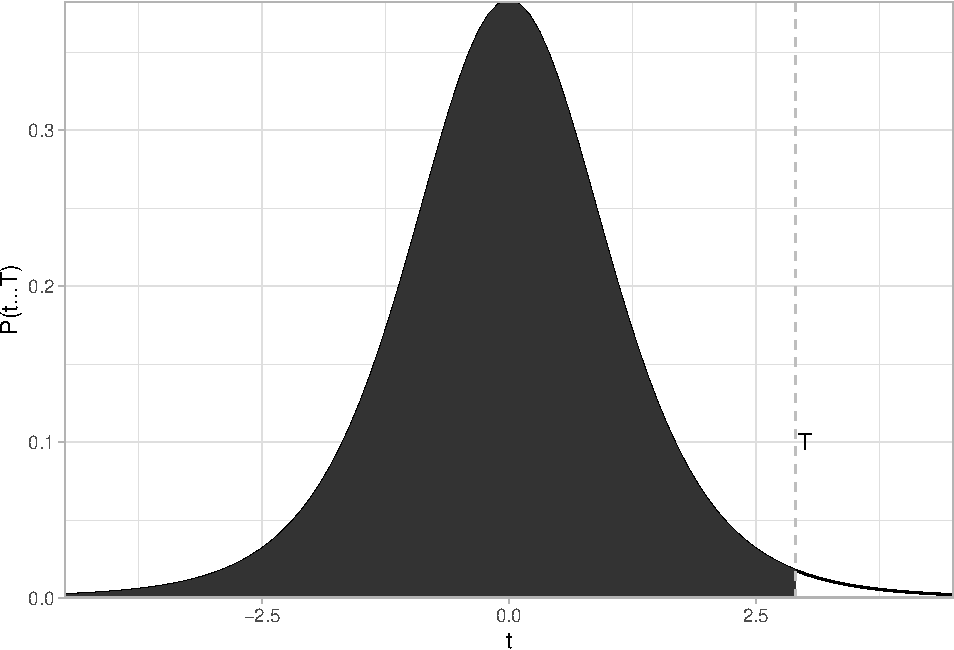
\includegraphics{R与tidyverse——数据分析入门_files/figure-latex/unnamed-chunk-59-1.pdf}

阴影面积为\(P(t<T)\),虚线对应的\(t\)为\(T\).
\texttt{qt()}可以把\(P(t≤T)\)的值转化成\(T\),\texttt{pt()}则相反。

假设你需要算一个confidence interval(置信区间),confidence level(置信等级)为\(95\%\),即\(\alpha=0.05\),degrees of freedom(自由度)为\(12\),那么怎么算\(t^*\)呢?

\begin{Shaded}
\begin{Highlighting}[]
\KeywordTok{qt}\NormalTok{(}\FloatTok{0.975}\NormalTok{, }\DataTypeTok{df =} \DecValTok{12}\NormalTok{)}
\end{Highlighting}
\end{Shaded}

\begin{verbatim}
## [1] 2.178813
\end{verbatim}

为什么是\(0.975\)?因为你要把\(0.05\)分到左右两边,所对应的t*就等同于t分布中,\(P(t ≤ T) = 0.975\)时T的值。

再举一个例子,你在做t检验,双尾的,算出来\(t=1.345\),自由度是\(15\),那么\(p\)值怎么算呢?

\begin{Shaded}
\begin{Highlighting}[]
\NormalTok{p <-}\StringTok{ }\NormalTok{(}\DecValTok{1}\OperatorTok{-}\NormalTok{(}\KeywordTok{pt}\NormalTok{(}\FloatTok{2.2}\NormalTok{, }\DataTypeTok{df =} \DecValTok{15}\NormalTok{)))}\OperatorTok{*}\DecValTok{2}
\NormalTok{p}
\end{Highlighting}
\end{Shaded}

\begin{verbatim}
## [1] 0.04389558
\end{verbatim}

其中\texttt{pt(2.2,\ df\ =\ 15)}算出阴影面积(\(P(t≤T)\)的值),1减去它再乘以2就是对应的双尾t检验的\(p\)值。

\hypertarget{z}{%
\subsection{z分布}\label{z}}

没有z分布专门的函数。可以直接用t分布代替,把\texttt{df}调到很大(比如\texttt{999999})就行了。比如我们试一下\(95\%\)置信区间所对应的\(z*\):

\begin{Shaded}
\begin{Highlighting}[]
\KeywordTok{qt}\NormalTok{(}\FloatTok{0.975}\NormalTok{,}\DecValTok{9999999}\NormalTok{)}
\end{Highlighting}
\end{Shaded}

\begin{verbatim}
## [1] 1.959964
\end{verbatim}

(果然是\(1.96\))

\hypertarget{t}{%
\subsection{t检验}\label{t}}

t检验分为以下几种:

\begin{itemize}
\tightlist
\item
  One sample t test (单样本)
\item
  paired t test(配对)
\item
  Two sample\ldots{}(双样本)

  \begin{itemize}
  \tightlist
  \item
    Unequal variance (Welch) t test(不等方差)
  \item
    Equal variance t test(等方差)
  \end{itemize}
\end{itemize}

在R中做t检验,很简单,以上这些t检验,都是用\texttt{t.test} 这个函数去完成。

以单样本为例:

\begin{Shaded}
\begin{Highlighting}[]
\NormalTok{x <-}\StringTok{ }\KeywordTok{c}\NormalTok{(}\FloatTok{2.23}\NormalTok{,}\FloatTok{2.24}\NormalTok{,}\FloatTok{2.34}\NormalTok{,}\FloatTok{2.31}\NormalTok{,}\FloatTok{2.35}\NormalTok{,}\FloatTok{2.27}\NormalTok{,}\FloatTok{2.29}\NormalTok{,}\FloatTok{2.26}\NormalTok{,}\FloatTok{2.25}\NormalTok{,}\FloatTok{2.21}\NormalTok{,}\FloatTok{2.29}\NormalTok{,}\FloatTok{2.34}\NormalTok{,}\FloatTok{2.32}\NormalTok{)}
\KeywordTok{t.test}\NormalTok{(x, }\DataTypeTok{mu =} \FloatTok{2.31}\NormalTok{)}
\end{Highlighting}
\end{Shaded}

\begin{verbatim}
## 
##  One Sample t-test
## 
## data:  x
## t = -2.0083, df = 12, p-value = 0.06766
## alternative hypothesis: true mean is not equal to 2.31
## 95 percent confidence interval:
##  2.257076 2.312155
## sample estimates:
## mean of x 
##  2.284615
\end{verbatim}

可以看到\(p=0.06766\)。

R的默认是双尾检验,你也可以设置成单尾的:

\begin{Shaded}
\begin{Highlighting}[]
\NormalTok{x <-}\StringTok{ }\KeywordTok{c}\NormalTok{(}\FloatTok{2.23}\NormalTok{,}\FloatTok{2.24}\NormalTok{,}\FloatTok{2.34}\NormalTok{,}\FloatTok{2.31}\NormalTok{,}\FloatTok{2.35}\NormalTok{,}\FloatTok{2.27}\NormalTok{,}\FloatTok{2.29}\NormalTok{,}\FloatTok{2.26}\NormalTok{,}\FloatTok{2.25}\NormalTok{,}\FloatTok{2.21}\NormalTok{,}\FloatTok{2.29}\NormalTok{,}\FloatTok{2.34}\NormalTok{,}\FloatTok{2.32}\NormalTok{)}

\KeywordTok{t.test}\NormalTok{(x, }\DataTypeTok{mu =} \FloatTok{2.31}\NormalTok{, }\DataTypeTok{alternative =} \StringTok{"less"}\NormalTok{) }\CommentTok{# 检验是否*less* than μ}
\end{Highlighting}
\end{Shaded}

\begin{verbatim}
## 
##  One Sample t-test
## 
## data:  x
## t = -2.0083, df = 12, p-value = 0.03383
## alternative hypothesis: true mean is less than 2.31
## 95 percent confidence interval:
##      -Inf 2.307143
## sample estimates:
## mean of x 
##  2.284615
\end{verbatim}

\(p\)值瞬间减半。

双样本/配对:

\begin{Shaded}
\begin{Highlighting}[]
\NormalTok{x <-}\StringTok{ }\KeywordTok{c}\NormalTok{(}\FloatTok{2.23}\NormalTok{,}\FloatTok{2.24}\NormalTok{,}\FloatTok{2.34}\NormalTok{,}\FloatTok{2.31}\NormalTok{,}\FloatTok{2.35}\NormalTok{,}\FloatTok{2.27}\NormalTok{,}\FloatTok{2.29}\NormalTok{,}\FloatTok{2.26}\NormalTok{,}\FloatTok{2.25}\NormalTok{,}\FloatTok{2.21}\NormalTok{,}\FloatTok{2.29}\NormalTok{,}\FloatTok{2.34}\NormalTok{,}\FloatTok{2.32}\NormalTok{)}
\NormalTok{y <-}\StringTok{ }\KeywordTok{c}\NormalTok{(}\FloatTok{2.27}\NormalTok{,}\FloatTok{2.29}\NormalTok{,}\FloatTok{2.37}\NormalTok{,}\FloatTok{2.38}\NormalTok{,}\FloatTok{2.39}\NormalTok{,}\FloatTok{2.25}\NormalTok{,}\FloatTok{2.39}\NormalTok{,}\FloatTok{2.16}\NormalTok{,}\FloatTok{2.55}\NormalTok{,}\FloatTok{2.81}\NormalTok{,}\FloatTok{2.19}\NormalTok{,}\FloatTok{2.44}\NormalTok{,}\FloatTok{2.22}\NormalTok{)}

\KeywordTok{t.test}\NormalTok{(x, y)}
\end{Highlighting}
\end{Shaded}

\begin{verbatim}
## 
##  Welch Two Sample t-test
## 
## data:  x and y
## t = -1.5624, df = 13.65, p-value = 0.1411
## alternative hypothesis: true difference in means is not equal to 0
## 95 percent confidence interval:
##  -0.18460351  0.02921889
## sample estimates:
## mean of x mean of y 
##  2.284615  2.362308
\end{verbatim}

R的默认是non-paired, unequal variance,你可以通过增加\texttt{paired\ =\ TRUE},\texttt{var.equal\ =\ TRUE}这两个参数来改变它。

\begin{Shaded}
\begin{Highlighting}[]
\KeywordTok{t.test}\NormalTok{(x, y, }\DataTypeTok{paired =} \OtherTok{TRUE}\NormalTok{)}
\end{Highlighting}
\end{Shaded}

\begin{verbatim}
## 
##  Paired t-test
## 
## data:  x and y
## t = -1.4739, df = 12, p-value = 0.1662
## alternative hypothesis: true difference in means is not equal to 0
## 95 percent confidence interval:
##  -0.19253874  0.03715412
## sample estimates:
## mean of the differences 
##             -0.07769231
\end{verbatim}

\hypertarget{chi2-}{%
\subsection{\texorpdfstring{\(\chi^2\) 检验}{\textbackslash{}chi\^{}2 检验}}\label{chi2-}}

\(\chi^2\)检验有两种,goodness of fit test(适配度检验)和contigency table test/test of independence(列联表分析/独立性检验)。都是用\texttt{chisq.test()}函数去完成。

\subsubsection{适配度检验}

假设我们制造了一个有问题的骰子,使1至6朝上的概率分别为:

\begin{Shaded}
\begin{Highlighting}[]
\NormalTok{expected_probs <-}\StringTok{ }\KeywordTok{c}\NormalTok{(}\FloatTok{0.05}\NormalTok{, }\FloatTok{0.1}\NormalTok{, }\FloatTok{0.15}\NormalTok{, }\FloatTok{0.2}\NormalTok{, }\FloatTok{0.2}\NormalTok{, }\FloatTok{0.3}\NormalTok{)}
\end{Highlighting}
\end{Shaded}

然后我们投掷了100次,实际1至6朝上的次数分别为:

\begin{Shaded}
\begin{Highlighting}[]
\NormalTok{observed_vals <-}\StringTok{ }\KeywordTok{c}\NormalTok{(}\DecValTok{6}\NormalTok{, }\DecValTok{9}\NormalTok{, }\DecValTok{14}\NormalTok{, }\DecValTok{24}\NormalTok{, }\DecValTok{18}\NormalTok{, }\DecValTok{29}\NormalTok{)}
\end{Highlighting}
\end{Shaded}

通过\texttt{chisq.test()},检验实际的1至6朝上概率是否与预期有偏差:

\begin{Shaded}
\begin{Highlighting}[]
\KeywordTok{chisq.test}\NormalTok{(observed_vals, }\DataTypeTok{p =}\NormalTok{ expected_probs) }\CommentTok{# 参数p是指概率}
\end{Highlighting}
\end{Shaded}

\begin{verbatim}
## 
##  Chi-squared test for given probabilities
## 
## data:  observed_vals
## X-squared = 1.4, df = 5, p-value = 0.9243
\end{verbatim}

p值很大(远大于0.05),因此结论是骰子各面朝上的概率符合预期。

如果不指定p参数,默认为检测是否所有值相等(即骰子的所有面朝上的概率相等):

\begin{Shaded}
\begin{Highlighting}[]
\KeywordTok{chisq.test}\NormalTok{(observed_vals)}
\end{Highlighting}
\end{Shaded}

\begin{verbatim}
## 
##  Chi-squared test for given probabilities
## 
## data:  observed_vals
## X-squared = 23.24, df = 5, p-value = 0.0003037
\end{verbatim}

这时p值小于0.05. 得出``骰子各面朝上的概率不等''的结论。

\subsubsection{列联表分析/独立性检验}

假设我们有一组不同年级的学生参加社团的人数数据:

\begin{Shaded}
\begin{Highlighting}[]
\NormalTok{(社团参与 <-}\StringTok{ }\KeywordTok{matrix}\NormalTok{(}\KeywordTok{c}\NormalTok{(}\DecValTok{28}\NormalTok{,}\DecValTok{36}\NormalTok{,}\DecValTok{40}\NormalTok{,}\DecValTok{40}\NormalTok{,}\DecValTok{32}\NormalTok{,}\DecValTok{33}\NormalTok{,}\DecValTok{38}\NormalTok{,}\DecValTok{29}\NormalTok{,}\DecValTok{36}\NormalTok{), }\DataTypeTok{nrow =} \DecValTok{3}\NormalTok{, }\DataTypeTok{dimnames =} \KeywordTok{list}\NormalTok{(}\KeywordTok{c}\NormalTok{(}\StringTok{"一年级"}\NormalTok{, }\StringTok{"二年级"}\NormalTok{, }\StringTok{"三年级"}\NormalTok{), }\KeywordTok{c}\NormalTok{(}\StringTok{"棒球"}\NormalTok{, }\StringTok{"足球"}\NormalTok{, }\StringTok{"网球"}\NormalTok{))))}
\end{Highlighting}
\end{Shaded}

\begin{verbatim}
##        棒球 足球 网球
## 一年级   28   40   38
## 二年级   36   32   29
## 三年级   40   33   36
\end{verbatim}

我们想知道社团的参与,与所在年级是否是独立事件:

\begin{Shaded}
\begin{Highlighting}[]
\KeywordTok{chisq.test}\NormalTok{(社团参与)}
\end{Highlighting}
\end{Shaded}

\begin{verbatim}
## 
##  Pearson's Chi-squared test
## 
## data:  社团参与
## X-squared = 3.7587, df = 4, p-value = 0.4396
\end{verbatim}

p值不小于0.05,无法拒绝``社团的参与,与所在年级是独立事件''的虚无假设。

彩蛋:用R代码实现卡方分布的概率密度函数的图像:

\begin{Shaded}
\begin{Highlighting}[]
\CommentTok{#其实还可以更精简,但是为了易读性不得不牺牲一点精简度。}
\NormalTok{Z <-}\StringTok{ }\KeywordTok{matrix}\NormalTok{(}\KeywordTok{rep}\NormalTok{(}\KeywordTok{rnorm}\NormalTok{(}\DecValTok{1000000}\NormalTok{), }\DecValTok{6}\NormalTok{), }\DataTypeTok{nrow =} \DecValTok{6}\NormalTok{)}\OperatorTok{^}\DecValTok{2}

\NormalTok{X <-}\StringTok{ }\NormalTok{Z}\OperatorTok{^}\DecValTok{2}

\NormalTok{Q <-}\StringTok{ }\KeywordTok{matrix}\NormalTok{(}\DataTypeTok{nrow =} \DecValTok{6}\NormalTok{, }\DataTypeTok{ncol =} \DecValTok{1000000}\NormalTok{)}

\ControlFlowTok{for}\NormalTok{ (i }\ControlFlowTok{in}\NormalTok{ (}\DecValTok{1}\OperatorTok{+}\DecValTok{1}\NormalTok{)}\OperatorTok{:}\DecValTok{6}\NormalTok{) \{}
\NormalTok{  Q[}\DecValTok{1}\NormalTok{,] =}\StringTok{ }\NormalTok{Z[}\DecValTok{1}\NormalTok{,]}
\NormalTok{  Q[i,] =}\StringTok{ }\NormalTok{Q[(i}\DecValTok{-1}\NormalTok{),] }\OperatorTok{+}\StringTok{ }\NormalTok{Z[i,]}
\NormalTok{\}}

\KeywordTok{plot}\NormalTok{(}\OtherTok{NULL}\NormalTok{, }\DataTypeTok{xlim=}\KeywordTok{c}\NormalTok{(}\FloatTok{0.23}\NormalTok{,}\DecValTok{6}\NormalTok{), }\DataTypeTok{ylim =} \KeywordTok{c}\NormalTok{(}\DecValTok{0}\NormalTok{,}\DecValTok{1}\NormalTok{),}
     \DataTypeTok{main =} \KeywordTok{expression}\NormalTok{(}\KeywordTok{paste}\NormalTok{(}\StringTok{'X ~ '}\NormalTok{, chi}\OperatorTok{^}\StringTok{'2'}\NormalTok{, }\StringTok{'(k)'}\NormalTok{)), }
     \DataTypeTok{xlab =} \StringTok{"x"}\NormalTok{, }
     \DataTypeTok{ylab=} \KeywordTok{expression}\NormalTok{(f[k]}\OperatorTok{*}\StringTok{'(x)'}\NormalTok{)}
\NormalTok{    )}
\NormalTok{colors <-}\StringTok{ }\KeywordTok{c}\NormalTok{(}\StringTok{'blue'}\NormalTok{, }\StringTok{'black'}\NormalTok{, }\StringTok{'red'}\NormalTok{, }\StringTok{'green'}\NormalTok{, }\StringTok{'gray'}\NormalTok{, }\StringTok{'orange'}\NormalTok{)}
\ControlFlowTok{for}\NormalTok{ (i }\ControlFlowTok{in} \DecValTok{1}\OperatorTok{:}\DecValTok{6}\NormalTok{) \{}
  \KeywordTok{lines}\NormalTok{(}\KeywordTok{density}\NormalTok{(Q[i,]),}
        \DataTypeTok{col=}\NormalTok{colors[i],}
        \DataTypeTok{lwd=}\DecValTok{2}\NormalTok{)}
\NormalTok{\}}
\KeywordTok{legend}\NormalTok{(}\StringTok{'topright'}\NormalTok{,}\KeywordTok{c}\NormalTok{(}\StringTok{'k=1'}\NormalTok{,}\StringTok{'k=2'}\NormalTok{,}\StringTok{'k=3'}\NormalTok{,}\StringTok{'k=4'}\NormalTok{,}\StringTok{'k=5'}\NormalTok{,}\StringTok{'k=6'}\NormalTok{),}
       \DataTypeTok{fill =}\NormalTok{ colors)}
\end{Highlighting}
\end{Shaded}

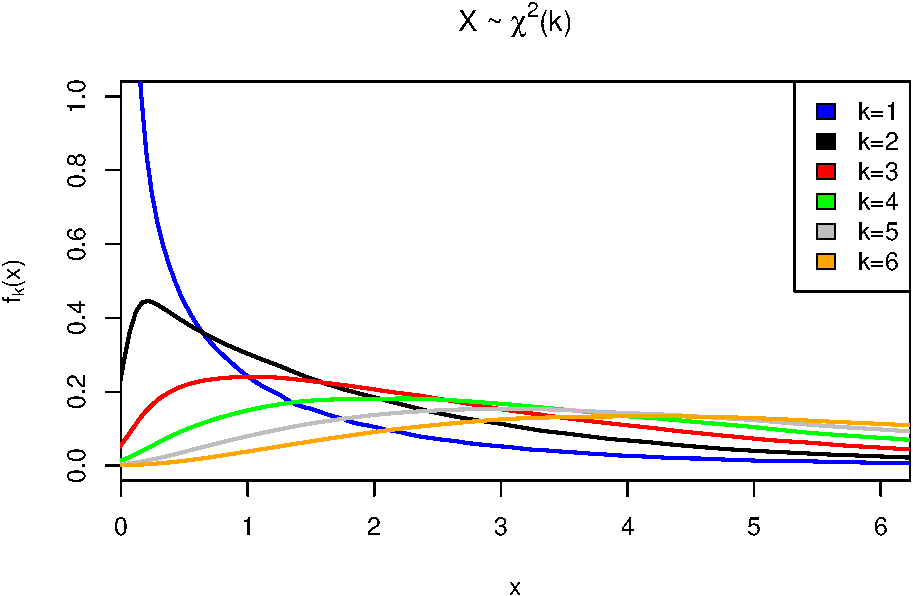
\includegraphics{R与tidyverse——数据分析入门_files/figure-latex/unnamed-chunk-73-1.pdf}

\hypertarget{-1}{%
\subsubsection{其它}\label{-1}}

R自带的检验还有\texttt{Box.test()}, \texttt{PP.test()}, \texttt{ansari.test()}, \texttt{bartlett.test()}, \texttt{wilcox.test}等共31种。查看帮助文件或利用网络资源以了解更多/

\hypertarget{tibble}{%
\chapter{dataframe(数据框)和tibble}\label{tibble}}

\hypertarget{dataframetibble}{%
\section{查看dataframe/tibble并了解它们的结构}\label{dataframetibble}}

\hypertarget{dataframetibble}{%
\subsection{dataframe/tibble的基本概念}\label{dataframetibble}}

dataframe是R中存储复杂数据的格式,它直观易操作。tibble是tidyverse的一部分,它是dataframe的进化版,功能更强大,更易操作。

我们来看个例子:

首先加载tidyverse:

\begin{Shaded}
\begin{Highlighting}[]
\KeywordTok{require}\NormalTok{(tidyverse)}
\end{Highlighting}
\end{Shaded}

\textbf{以后每次跟着本书使用R的时候,都要先加载tidyverse,不再重复提醒了。}

tidyverse中自带一些范例数据,比如我们输入:

\begin{Shaded}
\begin{Highlighting}[]
\NormalTok{mpg}
\end{Highlighting}
\end{Shaded}

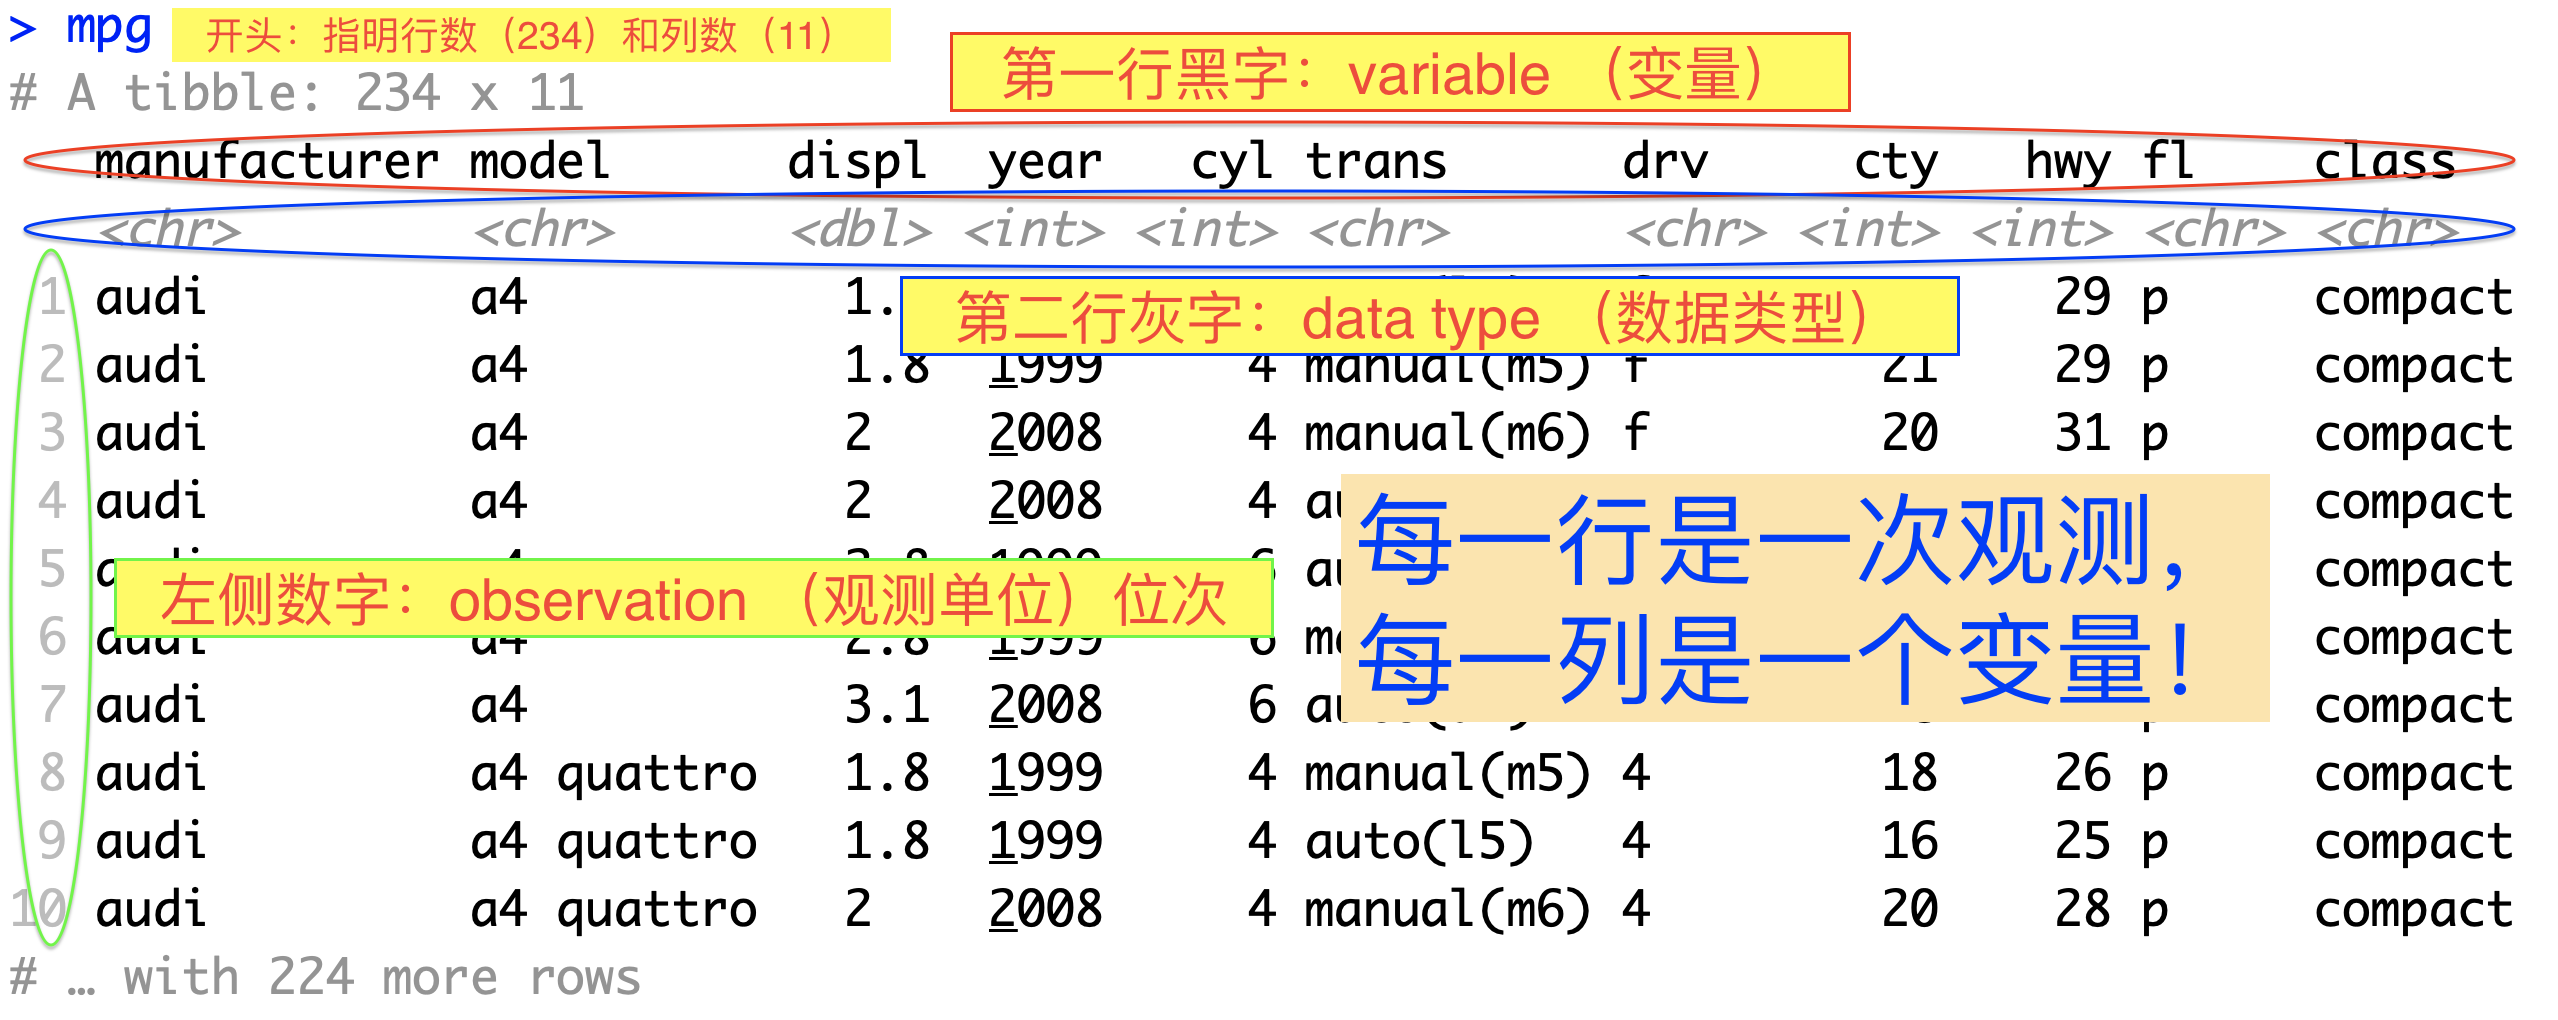
\includegraphics[width=35.53in]{img/tibble-intro}

这张图是重中之重。一个正确的dataframe/tibble,每一行代表的是一个observation(硬翻译的话是``观测单位'',但是我觉得这个翻译不好),每一列代表的是一个variable(变量),且同一个变量的数据类型必须一样\footnote{\url{https://thomaswdinsmore.com/2014/12/15/sas-versus-r-part-two/}}。像这样的数据被称为``tidy data''(``整齐的数据'')。虽然看起来简单,直观,理所当然,但是现实中上人们经常会做出``不整齐''的数据。把不整齐的数据弄整齐是下一章的重点。

\subsection{查看更多数据}

R默认显示dataframe/tibble的前10行。如果想看最后6行,可以使用\texttt{tail()}函数,比如:

\begin{Shaded}
\begin{Highlighting}[]
\KeywordTok{tail}\NormalTok{(mpg)}
\end{Highlighting}
\end{Shaded}

\begin{verbatim}
## # A tibble: 6 x 11
##   manufacturer model  displ  year   cyl trans drv     cty   hwy fl    class
##   <chr>        <chr>  <dbl> <int> <int> <chr> <chr> <int> <int> <chr> <chr>
## 1 volkswagen   passat   1.8  1999     4 auto~ f        18    29 p     mids~
## 2 volkswagen   passat   2    2008     4 auto~ f        19    28 p     mids~
## 3 volkswagen   passat   2    2008     4 manu~ f        21    29 p     mids~
## 4 volkswagen   passat   2.8  1999     6 auto~ f        16    26 p     mids~
## 5 volkswagen   passat   2.8  1999     6 manu~ f        18    26 p     mids~
## 6 volkswagen   passat   3.6  2008     6 auto~ f        17    26 p     mids~
\end{verbatim}

若要从头到尾查看全部数据,可以使用\texttt{View}函数:

\begin{Shaded}
\begin{Highlighting}[]
\KeywordTok{View}\NormalTok{(mpg)}
\end{Highlighting}
\end{Shaded}

\hypertarget{tibble}{%
\section{tibble的创建和基础操作}\label{tibble}}

\hypertarget{tibble}{%
\subsection{创建tibble}\label{tibble}}

\hypertarget{tibble}{%
\subsubsection{手动输入数据以创建tibble}\label{tibble}}

使用\texttt{tibble}函数,按以下格式创建tibble. 换行不是必须的,但是换行会看得更清楚。如果换行,不要忘记行末的逗号。

\begin{Shaded}
\begin{Highlighting}[]
\NormalTok{my_tibble_}\DecValTok{1}\NormalTok{ <-}\StringTok{ }\KeywordTok{tibble}\NormalTok{(}
                \DataTypeTok{nums =} \KeywordTok{c}\NormalTok{(}\DecValTok{4}\NormalTok{, }\DecValTok{5}\NormalTok{, }\DecValTok{6}\NormalTok{),}
                \DataTypeTok{chars =} \KeywordTok{c}\NormalTok{(}\StringTok{"hej"}\NormalTok{, }\StringTok{"你好"}\NormalTok{, }\StringTok{"こんにちは"}\NormalTok{),}
                \DataTypeTok{cplxnums =} \KeywordTok{c}\NormalTok{(}\StringTok{"4+8i"}\NormalTok{, }\StringTok{"3+5i"}\NormalTok{, }\StringTok{"3+4i"}\NormalTok{)}
\NormalTok{                )}
\NormalTok{my_tibble_}\DecValTok{1}
\end{Highlighting}
\end{Shaded}

\begin{verbatim}
## # A tibble: 3 x 3
##    nums chars      cplxnums
##   <dbl> <chr>      <chr>   
## 1     4 hej        4+8i    
## 2     5 你好       3+5i    
## 3     6 こんにちは 3+4i
\end{verbatim}

类似地,可以从现有的vector创建。\textbf{所有的变量长度必须一样。}

\begin{Shaded}
\begin{Highlighting}[]
\NormalTok{x <-}\StringTok{ }\KeywordTok{c}\NormalTok{(}\DecValTok{1}\NormalTok{,}\DecValTok{4}\NormalTok{,}\DecValTok{5}\NormalTok{)}
\NormalTok{y <-}\StringTok{ }\KeywordTok{c}\NormalTok{(}\DecValTok{211}\NormalTok{,}\DecValTok{23}\NormalTok{,}\DecValTok{45}\NormalTok{)}
\NormalTok{z <-}\StringTok{ }\KeywordTok{c}\NormalTok{(}\DecValTok{20}\NormalTok{,}\DecValTok{32}\NormalTok{)}
\end{Highlighting}
\end{Shaded}

\begin{Shaded}
\begin{Highlighting}[]
\NormalTok{my_tibble_}\DecValTok{2}\NormalTok{ <-}\StringTok{ }\KeywordTok{tibble}\NormalTok{(}\DataTypeTok{v1 =}\NormalTok{ x, }\DataTypeTok{v2 =}\NormalTok{ y)}
\NormalTok{my_tibble_}\DecValTok{2}
\end{Highlighting}
\end{Shaded}

\begin{verbatim}
## # A tibble: 3 x 2
##      v1    v2
##   <dbl> <dbl>
## 1     1   211
## 2     4    23
## 3     5    45
\end{verbatim}

而试图把\texttt{x}和\texttt{z}做成tibble就会报错:

\begin{Shaded}
\begin{Highlighting}[]
\NormalTok{my_tibble_}\DecValTok{3}\NormalTok{ <-}\StringTok{ }\KeywordTok{tibble}\NormalTok{(}\DataTypeTok{w1 =}\NormalTok{ x, }\DataTypeTok{w2 =}\NormalTok{ z)}

 \CommentTok{# Error: Tibble columns must have consistent lengths, only values of length one are recycled: * Length 2: Column `w2` * Length 3: Column `w1`}
\end{Highlighting}
\end{Shaded}

\hypertarget{dataframetibble}{%
\subsubsection{把dataframe转换成一个tibble}\label{dataframetibble}}

\begin{Shaded}
\begin{Highlighting}[]
\NormalTok{d1 <-}\StringTok{ }\KeywordTok{as.tibble}\NormalTok{(d) }\CommentTok{#其中d是一个dataframe}
\end{Highlighting}
\end{Shaded}

\hypertarget{tibble}{%
\subsubsection{从外部数据创建tibble}\label{tibble}}

参见第\ref{data-import}节(数据的导入)

\subsection{取子集(抓取行,列)}

\hypertarget{single-column}{%
\subsubsection{抓取单列}\label{single-column}}

抓取单列很简单,也很常用(比如我们只想从一个大的tibble中抓两个变量研究它们之间的关系)。 有两个符号可以用于抓取列,\texttt{\$}(仅用于变量名称)与\texttt{{[}{[}{]}{]}}(变量名称或索引)。还是以\texttt{mpg}为例,假设我们要抓取第3列 (\texttt{displ}):

\begin{Shaded}
\begin{Highlighting}[]
\CommentTok{########################}
\CommentTok{#通过变量名称抓取:}
\NormalTok{mpg[[}\StringTok{"displ"}\NormalTok{]]}
\CommentTok{#或}
\NormalTok{mpg}\OperatorTok{$}\NormalTok{displ }\CommentTok{#一般,在RStudio中此方法最方便,因为打出“$”之后会自动提示变量名。}

\CommentTok{########################}
\CommentTok{#通过索引抓取:}
\NormalTok{mpg[[}\DecValTok{3}\NormalTok{]]}
\end{Highlighting}
\end{Shaded}

以上三种方法都应得到同样的结果(是一个vector):

\begin{verbatim}
##  [1] 1.8 1.8 2.0 2.0 2.8 2.8 3.1 1.8 1.8 2.0 2.0 2.8 2.8 3.1 3.1 2.8 3.1
## [18] 4.2 5.3 5.3
\end{verbatim}

如果使用单方括号,得到的是一个tibble(试试\texttt{mpg{[}3{]}})这个特性在第\ref{dataframe-subsetting}节中有解释。

\subsubsection{抓取多列}

有时候,一个tibble中含有很多冗余信息,我们可能想把感兴趣的几个变量抓出来做一个新tibble. 这时\texttt{select()}函数最为方便。可以用变量名称或者索引来抓取。比如:

\begin{Shaded}
\begin{Highlighting}[]
\NormalTok{mpg_new <-}\StringTok{ }\KeywordTok{select}\NormalTok{(mpg, }\DecValTok{3}\OperatorTok{:}\DecValTok{5}\NormalTok{, }\DecValTok{8}\NormalTok{, }\DecValTok{9}\NormalTok{)}
\CommentTok{#等同于}
\NormalTok{mpg_new <-}\StringTok{ }\KeywordTok{select}\NormalTok{(mpg, displ, year, cyl, cty, hwy)}

\NormalTok{mpg_new}
\end{Highlighting}
\end{Shaded}

\begin{verbatim}
## # A tibble: 234 x 5
##    displ  year   cyl   cty   hwy
##    <dbl> <int> <int> <int> <int>
##  1   1.8  1999     4    18    29
##  2   1.8  1999     4    21    29
##  3   2    2008     4    20    31
##  4   2    2008     4    21    30
##  5   2.8  1999     6    16    26
##  6   2.8  1999     6    18    26
##  7   3.1  2008     6    18    27
##  8   1.8  1999     4    18    26
##  9   1.8  1999     4    16    25
## 10   2    2008     4    20    28
## # ... with 224 more rows
\end{verbatim}

base

\hypertarget{filter}{%
\subsubsection{\texorpdfstring{通过\texttt{filter()},抓取满足某条件的行}{通过filter(),抓取满足某条件的行}}\label{filter}}

通过\texttt{filter()},我们可以过滤出某个或多个变量满足某种条件的observations. 如果你还不熟悉逻辑运算,请看第\ref{logical-operations}节

假设我们只想看\texttt{mpg}中的奥迪品牌的,排量大于等于2且小于4的车辆的数据:

\begin{Shaded}
\begin{Highlighting}[]
\NormalTok{mpg_audi_displ2to4 <-}\StringTok{ }\KeywordTok{filter}\NormalTok{(mpg, manufacturer }\OperatorTok{==}\StringTok{ "audi"}\NormalTok{, displ }\OperatorTok{>=}\StringTok{ }\FloatTok{2.5} \OperatorTok{&}\StringTok{ }\NormalTok{displ }\OperatorTok{<}\StringTok{ }\DecValTok{4}\NormalTok{)}

\NormalTok{mpg_audi_displ2to4}
\end{Highlighting}
\end{Shaded}

\begin{verbatim}
## # A tibble: 9 x 11
##   manufacturer model  displ  year   cyl trans drv     cty   hwy fl    class
##   <chr>        <chr>  <dbl> <int> <int> <chr> <chr> <int> <int> <chr> <chr>
## 1 audi         a4       2.8  1999     6 auto~ f        16    26 p     comp~
## 2 audi         a4       2.8  1999     6 manu~ f        18    26 p     comp~
## 3 audi         a4       3.1  2008     6 auto~ f        18    27 p     comp~
## 4 audi         a4 qu~   2.8  1999     6 auto~ 4        15    25 p     comp~
## 5 audi         a4 qu~   2.8  1999     6 manu~ 4        17    25 p     comp~
## 6 audi         a4 qu~   3.1  2008     6 auto~ 4        17    25 p     comp~
## 7 audi         a4 qu~   3.1  2008     6 manu~ 4        15    25 p     comp~
## 8 audi         a6 qu~   2.8  1999     6 auto~ 4        15    24 p     mids~
## 9 audi         a6 qu~   3.1  2008     6 auto~ 4        17    25 p     mids~
\end{verbatim}

\hypertarget{slice}{%
\subsubsection{\texorpdfstring{用\texttt{slice()},通过行数(索引)抓取行。}{用slice(),通过行数(索引)抓取行。}}\label{slice}}

\begin{Shaded}
\begin{Highlighting}[]
\NormalTok{mpg_1to6 <-}\StringTok{ }\KeywordTok{slice}\NormalTok{(mpg, }\DecValTok{21}\OperatorTok{:}\DecValTok{26}\NormalTok{) }\CommentTok{# 抓取mpg的第21行至26行}
\NormalTok{mpg_1to6}
\end{Highlighting}
\end{Shaded}

\begin{verbatim}
## # A tibble: 6 x 11
##   manufacturer model  displ  year   cyl trans drv     cty   hwy fl    class
##   <chr>        <chr>  <dbl> <int> <int> <chr> <chr> <int> <int> <chr> <chr>
## 1 chevrolet    c1500~   5.3  2008     8 auto~ r        14    20 r     suv  
## 2 chevrolet    c1500~   5.7  1999     8 auto~ r        13    17 r     suv  
## 3 chevrolet    c1500~   6    2008     8 auto~ r        12    17 r     suv  
## 4 chevrolet    corve~   5.7  1999     8 manu~ r        16    26 p     2sea~
## 5 chevrolet    corve~   5.7  1999     8 auto~ r        15    23 p     2sea~
## 6 chevrolet    corve~   6.2  2008     8 manu~ r        16    26 p     2sea~
\end{verbatim}

我觉得\texttt{slice()}更实际的用途是随机选择个体:

\begin{Shaded}
\begin{Highlighting}[]
\NormalTok{mpg_random4 <-}\StringTok{ }\KeywordTok{slice}\NormalTok{(mpg, }\KeywordTok{sample}\NormalTok{(}\KeywordTok{length}\NormalTok{(mpg[[}\DecValTok{1}\NormalTok{]]), }\DecValTok{4}\NormalTok{)) }\CommentTok{# 随机四辆车}
\NormalTok{mpg_random4}
\end{Highlighting}
\end{Shaded}

\begin{verbatim}
## # A tibble: 4 x 11
##   manufacturer model  displ  year   cyl trans drv     cty   hwy fl    class
##   <chr>        <chr>  <dbl> <int> <int> <chr> <chr> <int> <int> <chr> <chr>
## 1 dodge        dakot~   3.7  2008     6 manu~ 4        15    19 r     pick~
## 2 land rover   range~   4.4  2008     8 auto~ 4        12    18 r     suv  
## 3 volkswagen   passat   1.8  1999     4 manu~ f        21    29 p     mids~
## 4 dodge        carav~   2.4  1999     4 auto~ f        18    24 r     mini~
\end{verbatim}

\hypertarget{factor}{%
\subsection{关于Factor}\label{factor}}

有时候,我们的变量是以文字的形式呈现,但是它们不是单纯的文字,而是有大小的差别,或是能以一定顺序排列,比如十二个月份 (Jan, Feb, \ldots{}),成绩的``优、良、中、差'',衣服的尺寸 (XS, S, M, XL, \ldots{}). 假设我们在做客户满意度调查,七位客户的反馈是

\begin{Shaded}
\begin{Highlighting}[]
\NormalTok{满意度_v <-}\StringTok{ }\KeywordTok{c}\NormalTok{(}\StringTok{"满意"}\NormalTok{, }\StringTok{"非常满意"}\NormalTok{, }\StringTok{"满意"}\NormalTok{, }\StringTok{"不满意"}\NormalTok{, }\StringTok{"满意"}\NormalTok{, }\StringTok{"非常不满"}\NormalTok{,  }\StringTok{"不满意"}\NormalTok{)}
\end{Highlighting}
\end{Shaded}

我们试图用\texttt{sort()}把七个反馈按满意度从小到大排列:

\begin{Shaded}
\begin{Highlighting}[]
\KeywordTok{sort}\NormalTok{(满意度_v)}
\end{Highlighting}
\end{Shaded}

\begin{verbatim}
## [1] "不满意"   "不满意"   "满意"     "满意"     "满意"     "非常不满"
## [7] "非常满意"
\end{verbatim}

可见其排序并不是有意义的。(因为默认英语根据'abcde\ldots{}'排序,中文根据笔画排序)

我们可以把这个vector做成factor,并用参数\texttt{levels}规定排序顺序:

\begin{Shaded}
\begin{Highlighting}[]
\CommentTok{# 按照惯例,小的值在前,大的在后;“非常不满”应为满意度最低的值。}
\NormalTok{满意度_f <-}\StringTok{ }\KeywordTok{factor}\NormalTok{(满意度_v, }\DataTypeTok{levels =} \KeywordTok{c}\NormalTok{(}\StringTok{"非常不满"}\NormalTok{, }\StringTok{"不满意"}\NormalTok{, }\StringTok{"满意"}\NormalTok{, }\StringTok{"非常满意"}\NormalTok{))}
\KeywordTok{sort}\NormalTok{(满意度_f)}
\end{Highlighting}
\end{Shaded}

\begin{verbatim}
## [1] 非常不满 不满意   不满意   满意     满意     满意     非常满意
## Levels: 非常不满 不满意 满意 非常满意
\end{verbatim}

这样排序就是正确的了。

\begin{Shaded}
\begin{Highlighting}[]
\KeywordTok{class}\NormalTok{(满意度_f) }\CommentTok{# "factor"}
\KeywordTok{is.vector}\NormalTok{(满意度_f) }\CommentTok{# FALSE}
\end{Highlighting}
\end{Shaded}

\hypertarget{list-arraymatrix}{%
\section{进阶内容:list, array和matrix}\label{list-arraymatrix}}

这一节为进阶内容,不用看。可以直接跳到下一章(第\ref{graphics}

其中的很多操作和dataframe或tibble中的操作是等效的。一般,tibble中的操作更直观,更容易上手。

\hypertarget{list}{%
\subsection{list(列表)简介}\label{list}}

R中的list是一种特殊的数据存储形式。使用\texttt{list()}函数来创建lists.

尝试对lists和vectors使用\texttt{is.vector()}, \texttt{is.list()}, \texttt{is.atomic()}和\texttt{is.recursive()}函数,你会发现list虽然也是``vector'',但我们一般说的``vector''都是指只能存储一种数据类型的atomic vector;而lists是recursive vector.

这意味着\textbf{一个list能存储多种类型的数据,且可以包含子list}。list中的每个元素是可以是一个(atomic) vector(如以下例子中的\texttt{{[}{[}1{]}{]}}和\texttt{{[}{[}3{]}{]}{[}{[}2{]}{]}}),也可以是一个list(如以下例子中的{[}{[}3{]}{]},它包含了有两个list元素的list;{[}{[}3{]}{]}是一个子list)。

\begin{Shaded}
\begin{Highlighting}[]
\NormalTok{y <-}\StringTok{ }\KeywordTok{list}\NormalTok{(}\DecValTok{1}\NormalTok{, }\KeywordTok{c}\NormalTok{(}\StringTok{"a"}\NormalTok{,}\StringTok{"あ"}\NormalTok{), }\KeywordTok{list}\NormalTok{(}\DecValTok{1}\OperatorTok{+}\NormalTok{3i, }\KeywordTok{c}\NormalTok{(}\OtherTok{FALSE}\NormalTok{, }\OtherTok{NA}\NormalTok{, }\OtherTok{TRUE}\NormalTok{)))}
\NormalTok{y}
\end{Highlighting}
\end{Shaded}

\begin{verbatim}
## [[1]]
## [1] 1
## 
## [[2]]
## [1] "a"  "あ"
## 
## [[3]]
## [[3]][[1]]
## [1] 1+3i
## 
## [[3]][[2]]
## [1] FALSE    NA  TRUE
\end{verbatim}

\hypertarget{list}{%
\subsubsection{list的索引/取子集}\label{list}}

使用上面的例子:

\begin{Shaded}
\begin{Highlighting}[]
\NormalTok{y[}\DecValTok{2}\NormalTok{] }\CommentTok{# 使用单方括号,得到的是一个只有一个list元素的list}
\end{Highlighting}
\end{Shaded}

\begin{verbatim}
## [[1]]
## [1] "a"  "あ"
\end{verbatim}

\begin{Shaded}
\begin{Highlighting}[]
\NormalTok{y[[}\DecValTok{2}\NormalTok{]] }\CommentTok{# 使用双方括号,得到的是一个vector}
\end{Highlighting}
\end{Shaded}

\begin{verbatim}
## [1] "a"  "あ"
\end{verbatim}

\begin{Shaded}
\begin{Highlighting}[]
\NormalTok{y[[}\DecValTok{3}\NormalTok{]][[}\DecValTok{2}\NormalTok{]] }\CommentTok{# 得到的也是一个vector;母list的索引在前,子list的在后}
\end{Highlighting}
\end{Shaded}

\begin{verbatim}
## [1] FALSE    NA  TRUE
\end{verbatim}

\begin{Shaded}
\begin{Highlighting}[]
\NormalTok{y[[}\DecValTok{3}\NormalTok{]] }\CommentTok{# 这个位置包含两个子list,因此得到一个有两个list元素的list}
\end{Highlighting}
\end{Shaded}

\begin{verbatim}
## [[1]]
## [1] 1+3i
## 
## [[2]]
## [1] FALSE    NA  TRUE
\end{verbatim}

\begin{Shaded}
\begin{Highlighting}[]
\NormalTok{y[[}\DecValTok{3}\NormalTok{]][[}\DecValTok{2}\NormalTok{]][}\DecValTok{2}\NormalTok{] }\CommentTok{# 得到vector时,直接在后面用单方括号}
\end{Highlighting}
\end{Shaded}

\begin{verbatim}
## [1] NA
\end{verbatim}

\hypertarget{dataframetibble}{%
\subsubsection{Dataframe和tibble的本质}\label{dataframetibble}}

聪明的你也许已经注意到了,dataframe/tibble\protect\hyperlink{single-column}{抓取单列的方法}和list的取子集惊人地相似(我曾经的语文老师喜欢调侃抄作业的同学的答案与参考答案``惊人地相似'')。

事实上,dataframe的本质正是list,而tibble也是dataframe(只是进化了一些功能):

\begin{Shaded}
\begin{Highlighting}[]
\KeywordTok{is.list}\NormalTok{(mpg)}
\end{Highlighting}
\end{Shaded}

\begin{verbatim}
## [1] TRUE
\end{verbatim}

\begin{Shaded}
\begin{Highlighting}[]
\KeywordTok{class}\NormalTok{(mpg)}
\end{Highlighting}
\end{Shaded}

\begin{verbatim}
## [1] "tbl_df"     "tbl"        "data.frame"
\end{verbatim}

\hypertarget{base-r-dataframe--tidyverse-tibble}{%
\subsection{Base R dataframe 和 Tidyverse tibble的区别}\label{base-r-dataframe--tidyverse-tibble}}

\hypertarget{dataframe-subsetting}{%
\subsubsection{Subsetting}\label{dataframe-subsetting}}

请查看\href{https://adv-r.hadley.nz/subsetting.html\#simplify-preserve}{Advanced R}了解更多。

\hypertarget{arraymatrix}{%
\subsection{array(数组)和matrix(矩阵)简介}\label{arraymatrix}}

Vector是一维的数据。Array是多维的数据。Matrix是二维的数据,因此matrix是array的一种特殊情况。

Dataframe不是matrix(虽然都是方的). Matrix是二维的,\textbf{仅包含数字}的\textbf{array}. Dataframe是一个二维的\textbf{list},不同列(即list元素)\textbf{可以存储不同的数据类型}。

我们可以用\texttt{dim()}来创建arrays:

\begin{Shaded}
\begin{Highlighting}[]
\NormalTok{A <-}\StringTok{ }\DecValTok{1}\OperatorTok{:}\DecValTok{48} \CommentTok{#创建一个(1,2,3,...24)的numeric vector}
\KeywordTok{dim}\NormalTok{(A) <-}\StringTok{ }\KeywordTok{c}\NormalTok{(}\DecValTok{6}\NormalTok{,}\DecValTok{8}\NormalTok{) }\CommentTok{#给A assign一个6乘4的dimensions}
\NormalTok{A}
\end{Highlighting}
\end{Shaded}

\begin{verbatim}
##      [,1] [,2] [,3] [,4] [,5] [,6] [,7] [,8]
## [1,]    1    7   13   19   25   31   37   43
## [2,]    2    8   14   20   26   32   38   44
## [3,]    3    9   15   21   27   33   39   45
## [4,]    4   10   16   22   28   34   40   46
## [5,]    5   11   17   23   29   35   41   47
## [6,]    6   12   18   24   30   36   42   48
\end{verbatim}

可以看到我们创建了一个二维的,array, 因此它也是一个(4行6列的)matrix。

\begin{Shaded}
\begin{Highlighting}[]
\KeywordTok{is.array}\NormalTok{(A)}
\end{Highlighting}
\end{Shaded}

\begin{verbatim}
## [1] TRUE
\end{verbatim}

\begin{Shaded}
\begin{Highlighting}[]
\KeywordTok{is.matrix}\NormalTok{(A)}
\end{Highlighting}
\end{Shaded}

\begin{verbatim}
## [1] TRUE
\end{verbatim}

注意24个数字排列的方式。第一个维度是行,所以先把4行排满,随后再使用下一个维度(列),使用第2列继续排4行,就像数字一样,(十进制中)先把个位从零数到9,再使用第二个位数(十位),以此类推。下面三维和四维的例子可能会更清晰。

同时注意最左边和最上边的{[}1,{]}, {[},3{]}之类的标记。你应该猜出来了,这些是index. 假设你要抓取第五行第三列的数值:

\begin{Shaded}
\begin{Highlighting}[]
\NormalTok{A[}\DecValTok{5}\NormalTok{,}\DecValTok{3}\NormalTok{]}
\end{Highlighting}
\end{Shaded}

\begin{verbatim}
## [1] 17
\end{verbatim}

或者第三行的全部数值:

\begin{Shaded}
\begin{Highlighting}[]
\NormalTok{A[}\DecValTok{3}\NormalTok{,]}
\end{Highlighting}
\end{Shaded}

\begin{verbatim}
## [1]  3  9 15 21 27 33 39 45
\end{verbatim}

或者第四列的全部数值:

\begin{Shaded}
\begin{Highlighting}[]
\NormalTok{A[,}\DecValTok{4}\NormalTok{]}
\end{Highlighting}
\end{Shaded}

\begin{verbatim}
## [1] 19 20 21 22 23 24
\end{verbatim}

接下来我们再看一个三维的例子(还是用1-48):

\begin{Shaded}
\begin{Highlighting}[]
\KeywordTok{dim}\NormalTok{(A) <-}\StringTok{ }\KeywordTok{c}\NormalTok{(}\DecValTok{2}\NormalTok{,}\DecValTok{8}\NormalTok{,}\DecValTok{3}\NormalTok{)}
\NormalTok{A}
\end{Highlighting}
\end{Shaded}

\begin{verbatim}
## , , 1
## 
##      [,1] [,2] [,3] [,4] [,5] [,6] [,7] [,8]
## [1,]    1    3    5    7    9   11   13   15
## [2,]    2    4    6    8   10   12   14   16
## 
## , , 2
## 
##      [,1] [,2] [,3] [,4] [,5] [,6] [,7] [,8]
## [1,]   17   19   21   23   25   27   29   31
## [2,]   18   20   22   24   26   28   30   32
## 
## , , 3
## 
##      [,1] [,2] [,3] [,4] [,5] [,6] [,7] [,8]
## [1,]   33   35   37   39   41   43   45   47
## [2,]   34   36   38   40   42   44   46   48
\end{verbatim}

它生成了三个二维的矩阵。在每个2*8的矩阵存储满16个元素后,第三个维度就要加一了。每个矩阵开头的\texttt{,\ ,\ x}正是第三个维度的值。同理,我们可以生成四维的array:

\begin{Shaded}
\begin{Highlighting}[]
\KeywordTok{dim}\NormalTok{(A) <-}\StringTok{ }\KeywordTok{c}\NormalTok{(}\DecValTok{3}\NormalTok{,}\DecValTok{4}\NormalTok{,}\DecValTok{2}\NormalTok{,}\DecValTok{2}\NormalTok{)}
\NormalTok{A}
\end{Highlighting}
\end{Shaded}

\begin{verbatim}
## , , 1, 1
## 
##      [,1] [,2] [,3] [,4]
## [1,]    1    4    7   10
## [2,]    2    5    8   11
## [3,]    3    6    9   12
## 
## , , 2, 1
## 
##      [,1] [,2] [,3] [,4]
## [1,]   13   16   19   22
## [2,]   14   17   20   23
## [3,]   15   18   21   24
## 
## , , 1, 2
## 
##      [,1] [,2] [,3] [,4]
## [1,]   25   28   31   34
## [2,]   26   29   32   35
## [3,]   27   30   33   36
## 
## , , 2, 2
## 
##      [,1] [,2] [,3] [,4]
## [1,]   37   40   43   46
## [2,]   38   41   44   47
## [3,]   39   42   45   48
\end{verbatim}

观察每个矩阵开头的\texttt{,\ ,\ x,\ y}. x是第三个维度,y是第四个维度。每个二位矩阵存满后,第三个维度(x)加一。x达到上限后,第四个维度(y)再加一。

类似二维矩阵,你可以通过index任意抓取数据,比如:

\begin{Shaded}
\begin{Highlighting}[]
\NormalTok{A[ ,}\DecValTok{3}\NormalTok{ , , ] }\CommentTok{#每个矩阵第3列的数据,即所有第二个维度为3的数值}
\end{Highlighting}
\end{Shaded}

\begin{verbatim}
## , , 1
## 
##      [,1] [,2]
## [1,]    7   19
## [2,]    8   20
## [3,]    9   21
## 
## , , 2
## 
##      [,1] [,2]
## [1,]   31   43
## [2,]   32   44
## [3,]   33   45
\end{verbatim}

\hypertarget{matricesarrays}{%
\subsection{给matrices和arrays命名}\label{matricesarrays}}

假设我们记录了3种药物(chloroquine, artemisinin, doxycycline)
对5种疟原虫(P. falciparum, P. malariae, P. ovale, P. vivax, P. knowlesi)的疗效,其中每个药物对每种疟原虫做6次实验。为了记录数据,我们可以做3个6*5的矩阵:(这里只是举例子,用的是随机生成的数字)

\begin{Shaded}
\begin{Highlighting}[]
\NormalTok{B <-}\StringTok{ }\KeywordTok{runif}\NormalTok{(}\DecValTok{90}\NormalTok{, }\DecValTok{0}\NormalTok{, }\DecValTok{1}\NormalTok{) }\CommentTok{#从均匀分布中取100个0到1之间的数}
\KeywordTok{dim}\NormalTok{(B) <-}\StringTok{ }\KeywordTok{c}\NormalTok{(}\DecValTok{6}\NormalTok{, }\DecValTok{5}\NormalTok{, }\DecValTok{3}\NormalTok{) }\CommentTok{#注意顺序}
\NormalTok{B}
\end{Highlighting}
\end{Shaded}

\begin{verbatim}
## , , 1
## 
##           [,1]       [,2]      [,3]       [,4]      [,5]
## [1,] 0.2733328 0.55216833 0.2414834 0.17121533 0.4099636
## [2,] 0.7684922 0.12266266 0.9883322 0.28112454 0.2438085
## [3,] 0.3333403 0.91729563 0.9449892 0.75163812 0.2076522
## [4,] 0.3293185 0.82260952 0.3200493 0.03729585 0.2311832
## [5,] 0.7770377 0.64489886 0.7179226 0.91205527 0.8527781
## [6,] 0.5006249 0.01798556 0.1103572 0.23300807 0.7673886
## 
## , , 2
## 
##            [,1]      [,2]       [,3]      [,4]      [,5]
## [1,] 0.03168819 0.9358690 0.30319995 0.8111589 0.4821811
## [2,] 0.68437211 0.9767348 0.93120194 0.7343984 0.7931656
## [3,] 0.09698453 0.9391623 0.08573336 0.1064778 0.1418348
## [4,] 0.01410627 0.8535771 0.11346088 0.1066444 0.1656295
## [5,] 0.14722911 0.3634736 0.32963875 0.0399176 0.8894229
## [6,] 0.85356769 0.9552780 0.33517983 0.2251467 0.1432204
## 
## , , 3
## 
##           [,1]      [,2]      [,3]      [,4]      [,5]
## [1,] 0.2292650 0.3607208 0.9184092 0.9354233 0.5562962
## [2,] 0.2181959 0.5978566 0.3005676 0.3990182 0.4547201
## [3,] 0.1544659 0.8980517 0.3700370 0.9026410 0.2504877
## [4,] 0.5162325 0.3463473 0.1741535 0.2305774 0.9751043
## [5,] 0.9737084 0.1882738 0.1466204 0.1805194 0.5386562
## [6,] 0.2281510 0.3142199 0.4600185 0.2674532 0.2398798
\end{verbatim}

然后我们用\texttt{dimnames()}来命名:

\begin{Shaded}
\begin{Highlighting}[]
\KeywordTok{dimnames}\NormalTok{(B) <-}\StringTok{ }\KeywordTok{list}\NormalTok{(}\KeywordTok{paste}\NormalTok{(}\StringTok{"trial."}\NormalTok{, }\DecValTok{1}\OperatorTok{:}\DecValTok{6}\NormalTok{), }\KeywordTok{c}\NormalTok{(}\StringTok{'P. falciparum'}\NormalTok{, }\StringTok{'P. malariae'}\NormalTok{, }\StringTok{'P. ovale'}\NormalTok{, }\StringTok{'P. vivax'}\NormalTok{, }\StringTok{'P. knowlesi'}\NormalTok{), }\KeywordTok{c}\NormalTok{(}\StringTok{'chloroquine'}\NormalTok{, }\StringTok{'artemisinin'}\NormalTok{, }\StringTok{'doxycycline'}\NormalTok{))}
\NormalTok{B}
\end{Highlighting}
\end{Shaded}

\begin{verbatim}
## , , chloroquine
## 
##          P. falciparum P. malariae  P. ovale   P. vivax P. knowlesi
## trial. 1     0.2733328  0.55216833 0.2414834 0.17121533   0.4099636
## trial. 2     0.7684922  0.12266266 0.9883322 0.28112454   0.2438085
## trial. 3     0.3333403  0.91729563 0.9449892 0.75163812   0.2076522
## trial. 4     0.3293185  0.82260952 0.3200493 0.03729585   0.2311832
## trial. 5     0.7770377  0.64489886 0.7179226 0.91205527   0.8527781
## trial. 6     0.5006249  0.01798556 0.1103572 0.23300807   0.7673886
## 
## , , artemisinin
## 
##          P. falciparum P. malariae   P. ovale  P. vivax P. knowlesi
## trial. 1    0.03168819   0.9358690 0.30319995 0.8111589   0.4821811
## trial. 2    0.68437211   0.9767348 0.93120194 0.7343984   0.7931656
## trial. 3    0.09698453   0.9391623 0.08573336 0.1064778   0.1418348
## trial. 4    0.01410627   0.8535771 0.11346088 0.1066444   0.1656295
## trial. 5    0.14722911   0.3634736 0.32963875 0.0399176   0.8894229
## trial. 6    0.85356769   0.9552780 0.33517983 0.2251467   0.1432204
## 
## , , doxycycline
## 
##          P. falciparum P. malariae  P. ovale  P. vivax P. knowlesi
## trial. 1     0.2292650   0.3607208 0.9184092 0.9354233   0.5562962
## trial. 2     0.2181959   0.5978566 0.3005676 0.3990182   0.4547201
## trial. 3     0.1544659   0.8980517 0.3700370 0.9026410   0.2504877
## trial. 4     0.5162325   0.3463473 0.1741535 0.2305774   0.9751043
## trial. 5     0.9737084   0.1882738 0.1466204 0.1805194   0.5386562
## trial. 6     0.2281510   0.3142199 0.4600185 0.2674532   0.2398798
\end{verbatim}

\textbf{清清楚楚,一目了然。}

\hypertarget{apply}{%
\subsection{\texorpdfstring{\texttt{apply}}{apply}}\label{apply}}

\begin{Shaded}
\begin{Highlighting}[]
\KeywordTok{apply}\NormalTok{(A,}\DecValTok{1}\NormalTok{,sum)}
\end{Highlighting}
\end{Shaded}

\begin{verbatim}
## [1] 376 392 408
\end{verbatim}

\hypertarget{graphics}{%
\chapter{使用ggplot绘图}\label{graphics}}

若要了解更多,请阅读ggplot开发者本人所编写的\emph{ggplot2: Elegand Graphics for Data Analysis}(Wickham \protect\hyperlink{ref-Wickham2015ggplot2-Elegant-Gra}{2015})。

\section{哲理}

\section{基础}

\subsection{基本语法}

\subsection{图像类型}

\section{进阶}

\subsection{逐层作图}

\subsection{尺寸,轴,和图例}

\subsection{位置}

\subsection{背景/主题的修改}

\hypertarget{ggplot}{%
\subsection{与ggplot编程}\label{ggplot}}

\hypertarget{base-r}{%
\section{附:Base R中的作图}\label{base-r}}

\hypertarget{wrangle}{%
\chapter{数据处理}\label{wrangle}}

\hypertarget{untidy-datatidy-data}{%
\section{把``untidy data''整成``tidy data''}\label{untidy-datatidy-data}}

\hypertarget{untidy-data}{%
\subsection{``untidy data''的主要问题}\label{untidy-data}}

\subsection{解决方案}

\section{数据的导入和导出}

\hypertarget{data-import}{%
\subsection{导入}\label{data-import}}

\hypertarget{csv}{%
\subsubsection{csv}\label{csv}}

\hypertarget{excel}{%
\subsubsection{excel}\label{excel}}

\hypertarget{-2}{%
\subsubsection{其它}\label{-2}}

\subsection{导出}

\hypertarget{python}{%
\chapter{与Python的联合使用}\label{python}}

\hypertarget{rpython-reticulate}{%
\section{\texorpdfstring{在R中使用Python: \texttt{reticulate}}{在R中使用Python: reticulate}}\label{rpython-reticulate}}

\hypertarget{pythonr-rpy}{%
\section{\texorpdfstring{在Python中使用R: \texttt{rpy}}{在Python中使用R: rpy}}\label{pythonr-rpy}}

\hypertarget{beaker-notebook}{%
\section{Beaker Notebook}\label{beaker-notebook}}

\url{https://decisionstats.com/2015/12/07/decisionstats-interview-scott-draves-beaker-notebook/}

Inspired by Jupyter, Beaker Notebook allows you to switch from one language in one code block to another language in another code block in a streamlined way to pass shared objects (data)

\hypertarget{bibiolography}{%
\chapter*{Bibiolography}\label{bibiolography}}
\addcontentsline{toc}{chapter}{Bibiolography}

\hypertarget{refs}{}
\leavevmode\hypertarget{ref-Gentleman2009R-Programming-Bioinfo}{}%
Gentleman, Robert. 2009. \emph{R Programming for Bioinformatics}. Book. Boca Raton, FL: CRC Press.

\leavevmode\hypertarget{ref-Kernighan1988The-C-Programming-La}{}%
Kernighan, Brain W., and Ednnis M. Ritchie. 1988. \emph{The C Programming Language}. 2nd ed. Prentice Hall.

\leavevmode\hypertarget{ref-R-base}{}%
R Core Team. 2019. \emph{R: A Language and Environment for Statistical Computing}. Vienna, Austria: R Foundation for Statistical Computing. \url{https://www.R-project.org/}.

\leavevmode\hypertarget{ref-R-rstudio}{}%
RStudio Team. 2015. \emph{RStudio: Integrated Development Environment for R}. Boston, MA: RStudio, Inc. \url{http://www.rstudio.com/}.

\leavevmode\hypertarget{ref-Wickham2015ggplot2-Elegant-Gra}{}%
Wickham, Hadley. 2015. \emph{Ggplot2: Elegant Graphics for Data Analysis}. Use R! Springer.

\leavevmode\hypertarget{ref-R-tidyverse}{}%
---------. 2017. \emph{Tidyverse: Easily Install and Load the 'Tidyverse'}. \url{https://CRAN.R-project.org/package=tidyverse}.

\leavevmode\hypertarget{ref-Ziemann2016Gene-name-errors}{}%
Ziemann, Mark, Yotam Eren, and Assam El-Osta. 2016. ``Gene Name Errors Are Widespread in the Scientific Literature.'' Journal Article. \emph{Genome Biology} 17 (1): 177. \url{https://doi.org/10.1186/s13059-016-1044-7}.


\end{document}
